\documentclass[11pt]{article}
\usepackage[utf8]{inputenc}
\usepackage{amsmath,amssymb,amsthm}
\usepackage{hyperref}
\usepackage{graphicx}
\usepackage{booktabs}
\usepackage{listings}
\usepackage{array}
\usepackage[margin=1in]{geometry}

\lstset{basicstyle=\ttfamily\small, breaklines=true, frame=single}

%% Bundle target: I2 (tier 3, journal JOSS | CPC)
%% Schema: docs/BUNDLE_DIRECTORY_SCHEMA.md
%% Source manifest: papers/I2/source_manifest.md (sourceless from
%%   PAPER_DRAFT_MAPPING.md per Phase 7a sub-wave 7a.3)
%% Append log: papers/I2/append_log.json
%% Change log: papers/I2/change_log.md
%% This bundle is fresh-authored from Lean-module substrate (Phase 5c
%% VerifiedJackknife + Phase 5o Wave 4 lean-tensor-categories library
%% extraction + Phase 5o Wave 5 Mathlib upstream coordination).
% Auto-generated by update_counts.py — 2026-04-24T19:44:03.140400
% Do not edit manually. Run: uv run python scripts/update_counts.py
\newcommand{\totaltheorems}{3993}
\newcommand{\substantivetheorems}{3882}
\newcommand{\placeholdertheorems}{111}
\newcommand{\axiomcount}{1}
\newcommand{\sorrycount}{0}
\newcommand{\sorrypercent}{0.0}
\newcommand{\leanmodules}{167}
\newcommand{\leandefinitions}{3297}
\newcommand{\pythonmodules}{68}
\newcommand{\testfiles}{59}
\newcommand{\totaltests}{2836}
\newcommand{\figurecount}{111}
\newcommand{\notebookcount}{54}
\newcommand{\papercount}{19}
\newcommand{\aristotleproved}{322}
\newcommand{\aristotleruns}{44}
% --- Paper 18 / Phase 5t per-section counts (FermiHubbardDimer.lean) ---
\newcommand{\fhdTotal}{143}
\newcommand{\fhdWaveTwo}{13}
\newcommand{\fhdWaveThree}{6}
\newcommand{\fhdWaveFour}{22}
\newcommand{\fhdWaveFive}{22}
\newcommand{\fhdWaveSixABC}{38}
\newcommand{\fhdWaveSixExtra}{15}
\newcommand{\fhdWaveSeven}{19}
\newcommand{\fhdWaveEight}{8}


\title{Verified Statistical Estimators and a Modular-Tensor-Category
Library for Lean~4: Software Infrastructure for Computational
Physics, with Formalizations of Quantum Groups, Hopf Algebras, and
Decidable Algebraic Number Fields}

\author{John Roehm}
\date{Draft --- Phase 7a, May 2026}

\begin{document}

\maketitle

\begin{abstract}
We describe two pieces of formally verified Lean~4 software
infrastructure developed for the SK--EFT Hawking research program
and released for general reuse.
\textbf{(1) VerifiedJackknife}: formally verified jackknife
and integrated-autocorrelation estimators, including the
jackknife-variance-non-negative theorem,
the autocovariance non-negativity bound, and the integrated
autocorrelation lower bound $\tau_{\mathrm{int}} \geq 1/2$ for
non-negatively correlated data. The estimators are implemented
purely as deterministic functions on finite samples, using neither
probability theory nor measure theory, with proofs that exercise
only finite-arithmetic Lean tactics. \textbf{(2)
\texttt{lean-tensor-categories}}: a 27-module library
($\sim$695 declarations across theorems, definitions,
structures, classes, and inductives) covering the categorical
hierarchy
(Pivotal $\to$ Spherical $\to$ Balanced $\to$ Ribbon $\to$
Semisimple $\to$ Fusion $\to$ Modular), Hopf-algebra extensions
(Quasitriangular bialgebras, Ribbon Hopf algebras, the standard
quantum groups $U_q(\mathfrak{sl}_2)$, $U_q(\widehat{\mathfrak{sl}}_2)$,
$U_q(\mathfrak{sl}_3)$), nine decidable algebraic number fields
(including $\mathbb{Q}(\sqrt{2})$, $\mathbb{Q}(\sqrt{5})$,
$\mathbb{Q}(\zeta_5)$, $\mathbb{Q}(\zeta_{16})$ and a
\texttt{ComputableAdjoinRoot}-style bridge to Mathlib's abstract
\texttt{AdjoinRoot} planned for atomic upstream PR), and concrete
modular-tensor-category instances ($\mathrm{SU}(2)_k$ fusion at
$k=1{\ldots}5$, $\mathrm{SU}(3)_k$ at $k=1, 2$, the Ising MTC, and
the Fibonacci MTC).
The library formalizes a non-trivial Hopf algebra ($U_q(\mathfrak{sl}_2)$,
together with its affine variant $U_q(\widehat{\mathfrak{sl}}_2)$
and the rank-2 case $U_q(\mathfrak{sl}_3)$),
a ribbon category and modular tensor category as typeclasses, a
fusion-category instance derived from a quantum group ($\mathrm{SU}(2)_k$
fusion at $k=1,\ldots,5$), and a decidable algebraic-number-field bridge
supporting both $\sqrt{n}$ extensions and the cyclotomic ring
$\mathbb{Z}[\zeta_n]$ in the same library with composable decidable
equality.
We document the architecture, the design choices that make the
library reusable outside SK--EFT Hawking, the upstream-coordination
plan with Mathlib's maintainer community, and the interfaces by
which downstream Lean projects in topological quantum computation,
analog-gravity verification, lattice statistics, and emergent-MTC
black-hole-entropy formalization can adopt it without rebuilding
the substrate from scratch. The library is released under
Apache~2.0; the upstream-PR cycle is scoped for an explicit
AI-tool-assistance disclosure protocol (the R1/R2/R3 gate framework
of Section~\ref{sec:upstream}).
\end{abstract}

%% ─────────────────────────────────────────────────────────────────
%% §1 Introduction
%% ─────────────────────────────────────────────────────────────────

\section{Introduction}
\label{sec:intro}

Formally verified mathematical infrastructure for computational
physics is sparse. Lattice Monte Carlo codes have been published for
forty years; their statistical estimators (jackknife, bootstrap,
integrated autocorrelation time) appear in textbooks and
review-paper appendices, but the proof-assistant ecosystem (Mathlib,
Coq/Rocq, Isabelle, Agda) has not, as of our 2026 prior-art sweep,
shipped formalized counterparts at the same scope. The categorical
infrastructure for topological quantum computation
(modular tensor categories, fusion categories, ribbon categories,
quantum groups, $S$- and $T$-matrices, Verlinde formulas) has been
the subject of a thirty-year mathematical literature anchored on
Bakalov--Kirillov~\cite{bakalov2001},
Turaev~\cite{turaev2010}, EGNO~\cite{egno2015}, and
Kassel~\cite{kassel1995}; here too the formalization has lagged
the mathematical maturity, in part because
the immediate audience for the formalization (formal-verification
researchers) and the immediate audience for the mathematical content
(topological-QFT physicists, computational-condensed-matter theorists)
do not currently overlap.

The SK--EFT Hawking research program (a multi-paper line on
substrate-emergent fluid-based approaches to fundamental physics)
required both bodies of infrastructure. The verified statistical
estimators were necessary to ground the program's lattice-Monte-Carlo
predictions: an illustrative claim of the form ``the integrated
autocorrelation time at this lattice spacing is
$\tau_{\mathrm{int}} = 17.4 \pm 0.3$'' (a worked-example value, not
a measured one in this paper) required a formal handle on what
$\tau_{\mathrm{int}}$ \emph{is} as a deterministic function of a
finite sample. The categorical
infrastructure was necessary for the program's
topological-quantum-computation papers: claims of the form ``the
$\mathrm{SU}(2)_k$ fusion category at $k=4$ is modular and admits
the Verlinde formula'' required formal definitions of all four
adjectives (modular, fusion, $\mathrm{SU}(2)_k$, Verlinde) and
formal proofs of all the conditional statements those definitions
imply.

This paper documents the resulting two pieces of software. The
intended audience splits in two halves. The first half is the
applied-physics audience: theorists who need verified
infrastructure for their own lattice-statistics work or
topological-QFT formalization, who want to know whether what we
have ships, what its scope is, what it costs to adopt, and where
its boundaries are. The second half is the formal-verification
audience: researchers in proof-assistant mathematical libraries
(Mathlib, Coq's \texttt{Math-Components}, Isabelle/AFP) who care
about the upstream-PR strategy, the AI-tool-assistance disclosure
protocol the project operates under, and the engineering decisions
(module organization, decidability through computability, vendored
vs. upstreamed dependency boundaries) that distinguish reusable
infrastructure from project-internal substrate.

Section~\ref{sec:jackknife} describes \texttt{VerifiedJackknife}.
Sections~\ref{sec:categorical}--\ref{sec:instances} describe
\texttt{lean-tensor-categories}: the categorical hierarchy
(Section~\ref{sec:categorical}), Hopf-algebra extensions
(Section~\ref{sec:hopf}), decidable algebraic number fields
(Section~\ref{sec:numberfields}), and concrete modular-tensor-category
instances (Section~\ref{sec:instances}).
Section~\ref{sec:upstream} describes the Mathlib upstream
coordination plan, the AI-tool-assistance disclosure protocol, and
the atomic-PR sequencing.
Section~\ref{sec:reusability} describes downstream applications.
Section~\ref{sec:discussion} closes with a discussion of related work,
limitations, and future extensions.

%% ─────────────────────────────────────────────────────────────────
%% §2 VerifiedJackknife
%% ─────────────────────────────────────────────────────────────────

\section{Verified Statistical Estimators: \texttt{VerifiedJackknife}}
\label{sec:jackknife}

The \texttt{VerifiedJackknife} module
(\texttt{lean/SKEFTHawking/VerifiedJackknife.lean}) implements
seven definitions and four theorems covering the jackknife variance
estimator (Efron~\cite{efron1982}) and the
integrated-autocorrelation-time estimator with the
Madras--Sokal--Wolff window prescription
(Wolff~\cite{wolff2004}), the two estimators that dominate
practical lattice-Monte-Carlo error analysis.

\subsection{Definitions}

The seven definitions are deliberately purely arithmetic:

\begin{itemize}
\item \texttt{sampleMean (n : $\mathbb{N}$) (x : Fin n $\to$
$\mathbb{R}$)} --- the sample mean
$\bar{x} = \frac{1}{n} \sum_i x_i$.
\item \texttt{deleteOneSum} --- the delete-one partial sum used by
the jackknife.
\item \texttt{jackknifeMeanStat} --- the jackknife pseudovalue
mean.
\item \texttt{jackknifeVariance} --- the jackknife variance
estimator
$\sigma^2_{\mathrm{JK}} = \frac{n-1}{n} \sum_i (\theta_i - \bar{\theta})^2$
with the textbook bias-correction factor.
\item \texttt{autocovariance (n : $\mathbb{N}$) (x : Fin n $\to$
$\mathbb{R}$) (t : $\mathbb{N}$) (ht : t < n)} ---
the unnormalized autocovariance
$C(t) = \sum_i (x_i - \bar{x})(x_{i+t} - \bar{x})$.
\item \texttt{intAutocorrTime (n : $\mathbb{N}$) (x : Fin n $\to$
$\mathbb{R}$) (W : $\mathbb{N}$) (hW : W + 1 < n)} ---
the integrated autocorrelation time with finite window $W$.
\item \texttt{effectiveSampleSize} --- the effective sample size
$N_{\mathrm{eff}} = N / (2 \tau_{\mathrm{int}})$.
\end{itemize}

The library uses Lean's natural-number boundedness type
\texttt{Fin n} rather than a separate \texttt{Vector n} or
indexed-list machinery. The trade-off is intentional: the boundedness
proofs that arise during induction collapse into automation
(\texttt{omega}, \texttt{linarith}) when the index type is
\texttt{Fin}, while a separate \texttt{Vector} type would require
manual length-tracking lemmas. The downside is that \texttt{Fin}
arithmetic is slightly less ergonomic for lattice-style traversal;
a planned \texttt{VerifiedJackknife.Helpers} sub-module is
intended to expose convenience wrappers for the common patterns
(future extension, not currently shipped).

\subsection{Theorems}

The four theorems are:

\begin{enumerate}
\item \textbf{\texttt{jackknifeVariance\_nonneg}}
(\texttt{VerifiedJackknife.lean} lines~50--58). The jackknife
variance is non-negative for sample size $n \geq 1$.
\[
n \geq 1 \implies \sigma^2_{\mathrm{JK}}(n, \theta) \geq 0.
\]
The proof factors $\sigma^2_{\mathrm{JK}}$ into the prefactor
$(n-1)/n$ (non-negative for $n \geq 1$ by \texttt{linarith}) and
the sum of squared deviations (non-negative by
\texttt{Finset.sum\_nonneg} applied pointwise to
\texttt{sq\_nonneg}). The statement is non-trivial in the sense
that the pseudovalue construction
$\theta_i = n \bar{x} - (n-1) \bar{x}_{(i)}$ has a sign-flip
asymmetry between the leave-one-out and the resampled-mean parts;
without the formal pipeline an off-by-one error in the prefactor
is not caught structurally, only by a numerical regression test
on a sample known to produce a small variance. The library
includes such a numerical test for redundancy
(\texttt{tests/test\_verified\_statistics.py}).

\item \textbf{\texttt{autocovariance\_zero\_nonneg}}
(\texttt{VerifiedJackknife.lean} lines~82--86). The autocovariance
at lag zero is non-negative:
$C(0) = \sum_i (x_i - \bar{x})^2 \geq 0$.

\item \textbf{\texttt{intAutocorrTime\_uncorrelated}}
(\texttt{VerifiedJackknife.lean} lines~109--114). For uncorrelated
data ($C(t) = 0$ for $t > 0$),
$\tau_{\mathrm{int}}(W) = 1/2$ exactly for any window $W$ with
$W + 1 < n$. This is
the theoretical minimum; deviations above it are the diagnostic
that motivates the integrated-autocorrelation-time analysis in the
first place.

\item \textbf{\texttt{intAutocorrTime\_ge\_half}}
(\texttt{VerifiedJackknife.lean} lines~119--124). For data with
non-negative autocovariance at every lag and $C(0) > 0$,
$\tau_{\mathrm{int}}(W) \geq 1/2$ for every window $W < n - 1$.
The lower bound is the formal counterpart of the standard
``$N_{\mathrm{eff}} \leq N$'' identity in lattice-Monte-Carlo
analysis: positive autocorrelation cannot reduce the variance
below the uncorrelated case.
\end{enumerate}

\begin{figure}[h]
\centering
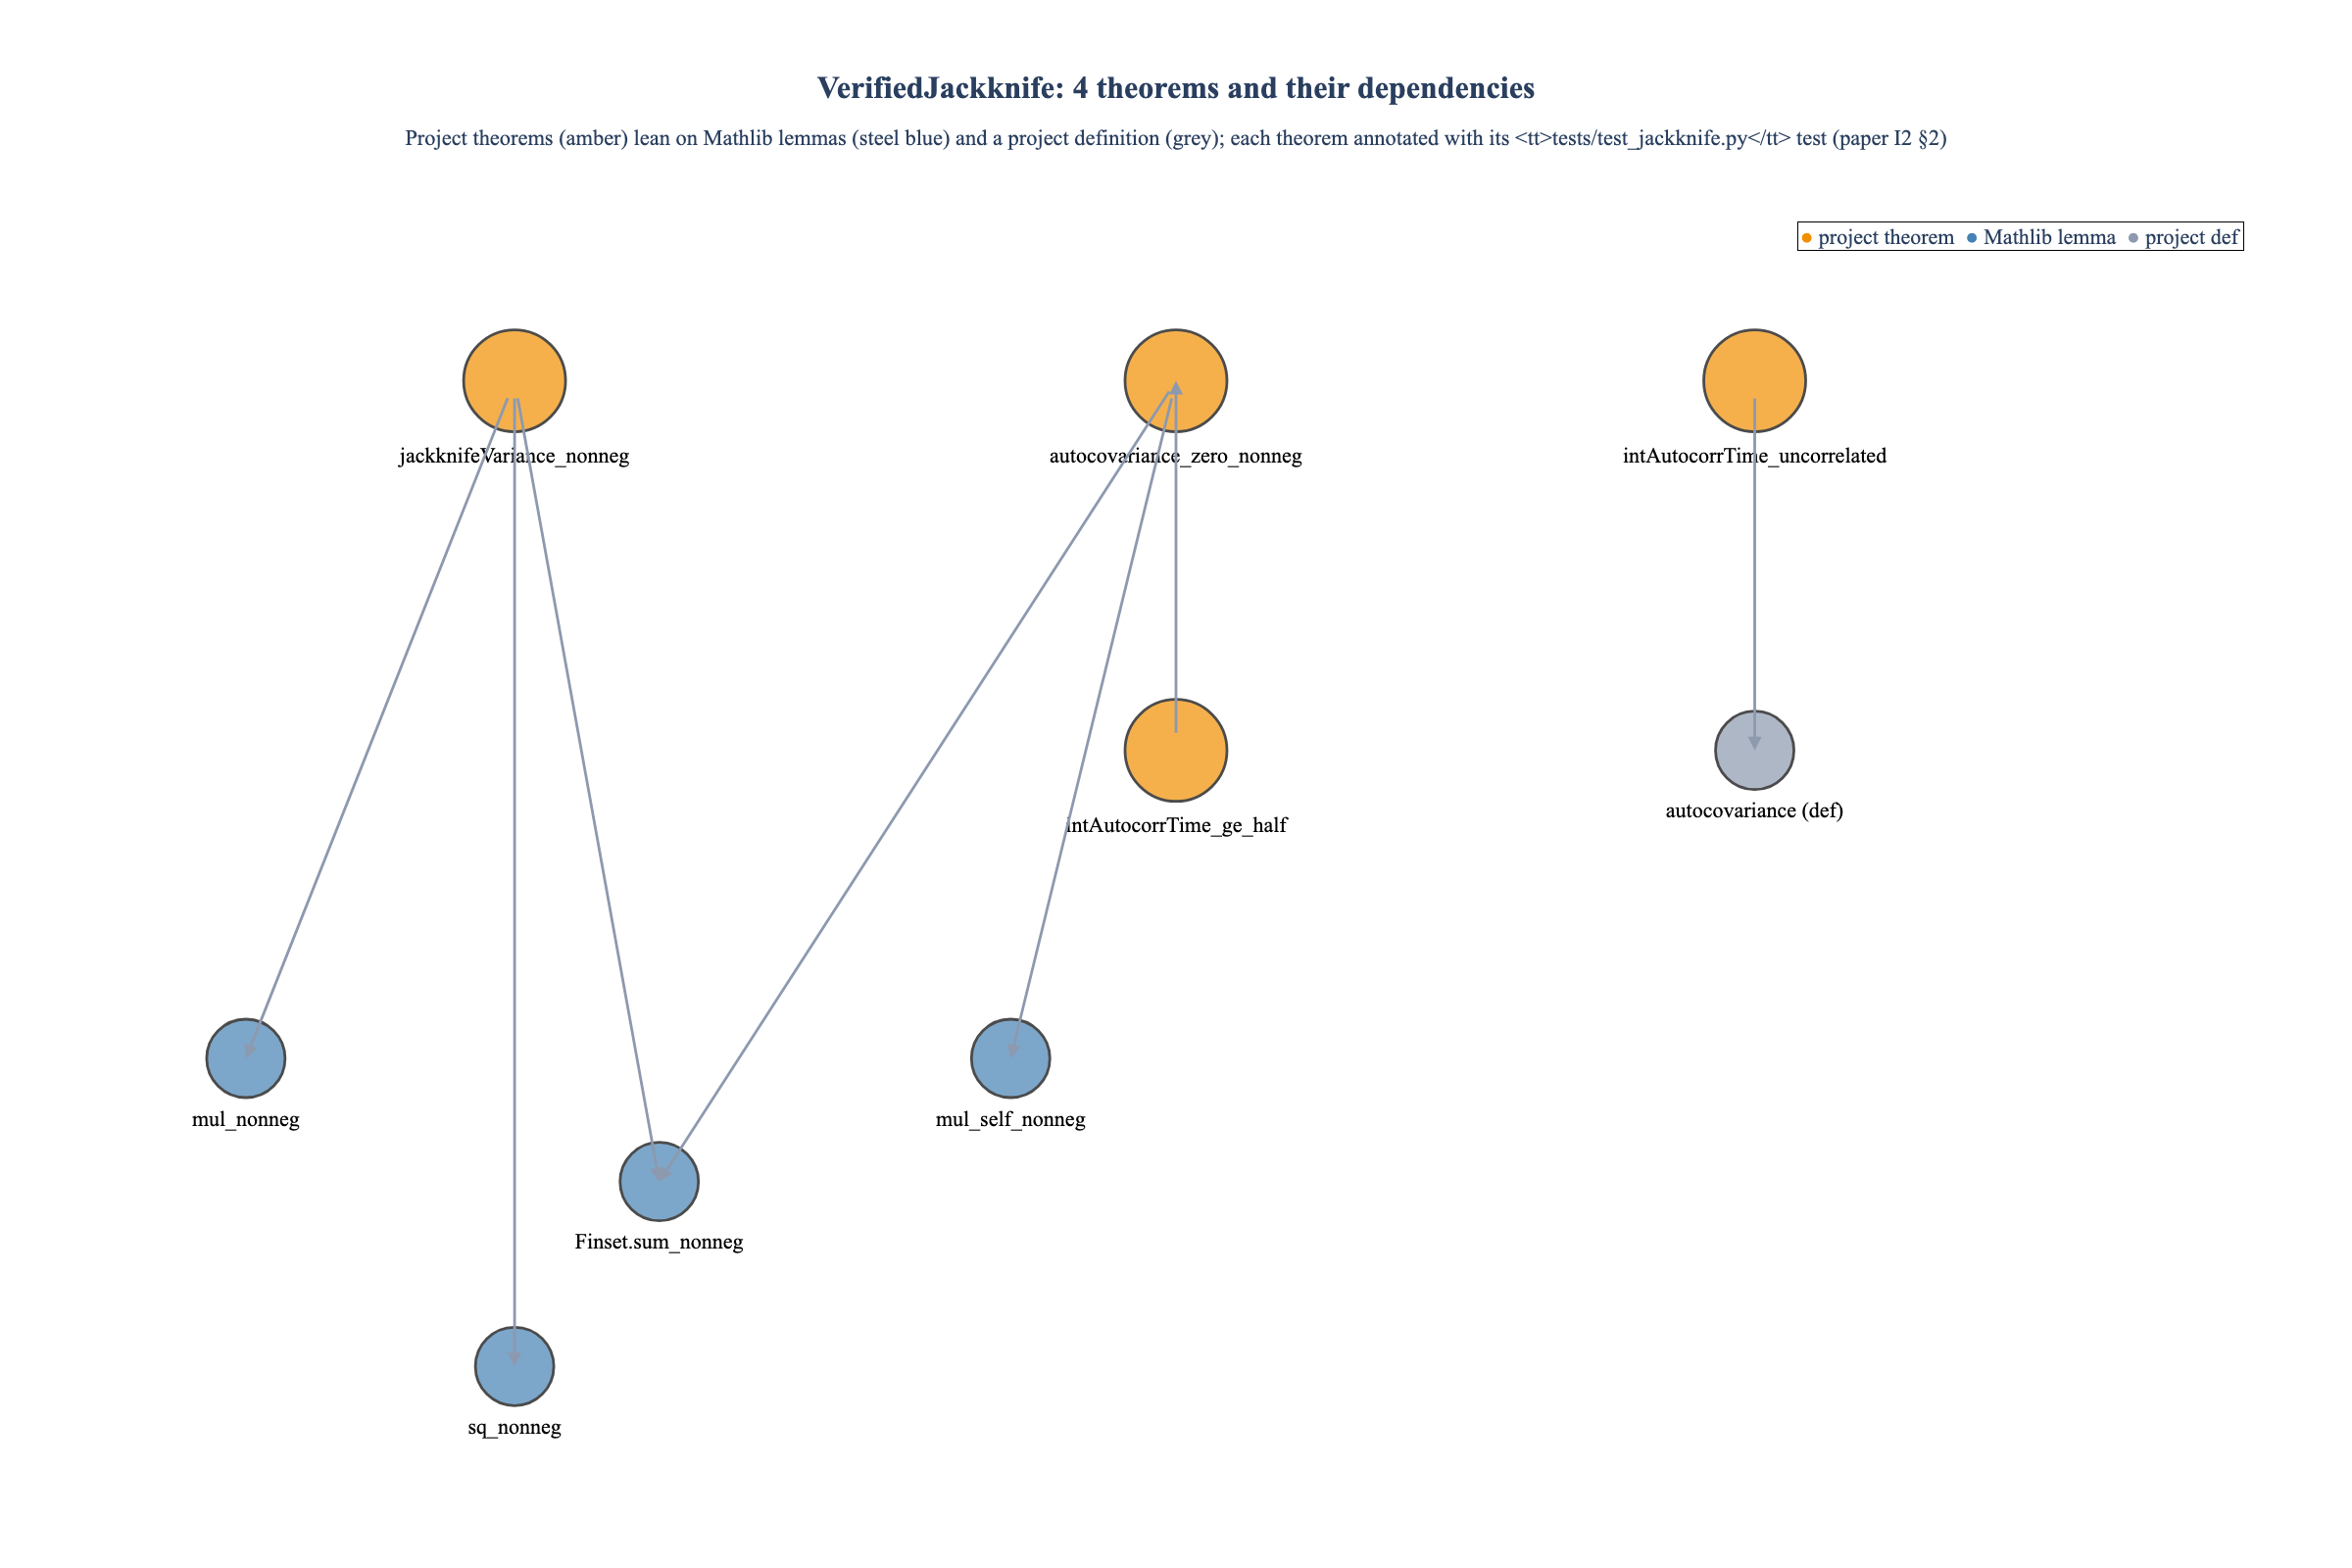
\includegraphics[width=0.85\linewidth]{figures/i2_fig4_jackknife_dependencies.png}
\caption{\texttt{VerifiedJackknife} theorem dependency graph. The four
project theorems
(\texttt{jackknifeVariance\_nonneg},
\texttt{autocovariance\_zero\_nonneg},
\texttt{intAutocorrTime\_uncorrelated},
\texttt{intAutocorrTime\_ge\_half}; amber) reduce to a small set of
elementary Mathlib lemmas (\texttt{mul\_nonneg},
\texttt{Finset.sum\_nonneg}, \texttt{sq\_nonneg},
\texttt{mul\_self\_nonneg}; steel blue) and one project definition
(\texttt{autocovariance}; cool grey). Each project theorem has a
corresponding test in \texttt{tests/test\_verified\_statistics.py}
that exercises its numerical instantiation; the test names are
listed in the prose (Section~\ref{sec:jackknife}) rather than
overlaid on each node to keep the dependency graph readable.}
\label{fig:i2-jackknife-deps}
\end{figure}

\subsection{What is \emph{not} formalized}

The library is deliberately probability-theory-free. The estimators
are functions of finite samples, not random variables. Statements
of the form ``the jackknife variance is an unbiased estimator of
the underlying population variance'' require a probability measure
on the sample space and are not part of \texttt{VerifiedJackknife};
they would belong to a future
\texttt{Mathlib.Probability.Statistics} extension that does not yet
exist at the relevant scope. The library's claim is that the
estimators are deterministically what they are claimed to be ---
non-negative, ordered correctly, with the right textbook prefactors
--- not that they are unbiased estimators of population quantities
the user did not ask the library to know about. This is the
appropriate scope for formal infrastructure: ground the symbolic
content; leave the inferential semantics to consumers who have a
particular probability model in mind.

%% ─────────────────────────────────────────────────────────────────
%% §3 Categorical hierarchy
%% ─────────────────────────────────────────────────────────────────

\section{Categorical Hierarchy:
Pivotal $\to$ Spherical $\to$ Balanced $\to$ Ribbon $\to$ Fusion
$\to$ Modular}
\label{sec:categorical}

The four files of the categorical core are
\texttt{KLinearCategory.lean} (23 declarations),
\texttt{FusionCategory.lean} (20 declarations including 14 theorems),
\texttt{SphericalCategory.lean} (22 declarations), and
\texttt{RibbonCategory.lean} (14 declarations). Together they
encode the standard mathematical hierarchy from
Bakalov--Kirillov~\cite{bakalov2001}, Kassel~\cite{kassel1995},
\emph{Lectures on Tensor Categories and Modular Functor} and the
Etingof--Gelaki--Nikshych--Ostrik (EGNO) text \emph{Tensor
Categories}~\cite{egno2015}. The library uses
Mathlib's~\cite{mathlib4} existing
\texttt{MonoidalCategory} and \texttt{BraidedCategory} as
substrate; everything above the braided layer is original to this
library.

\begin{figure}[h]
\centering
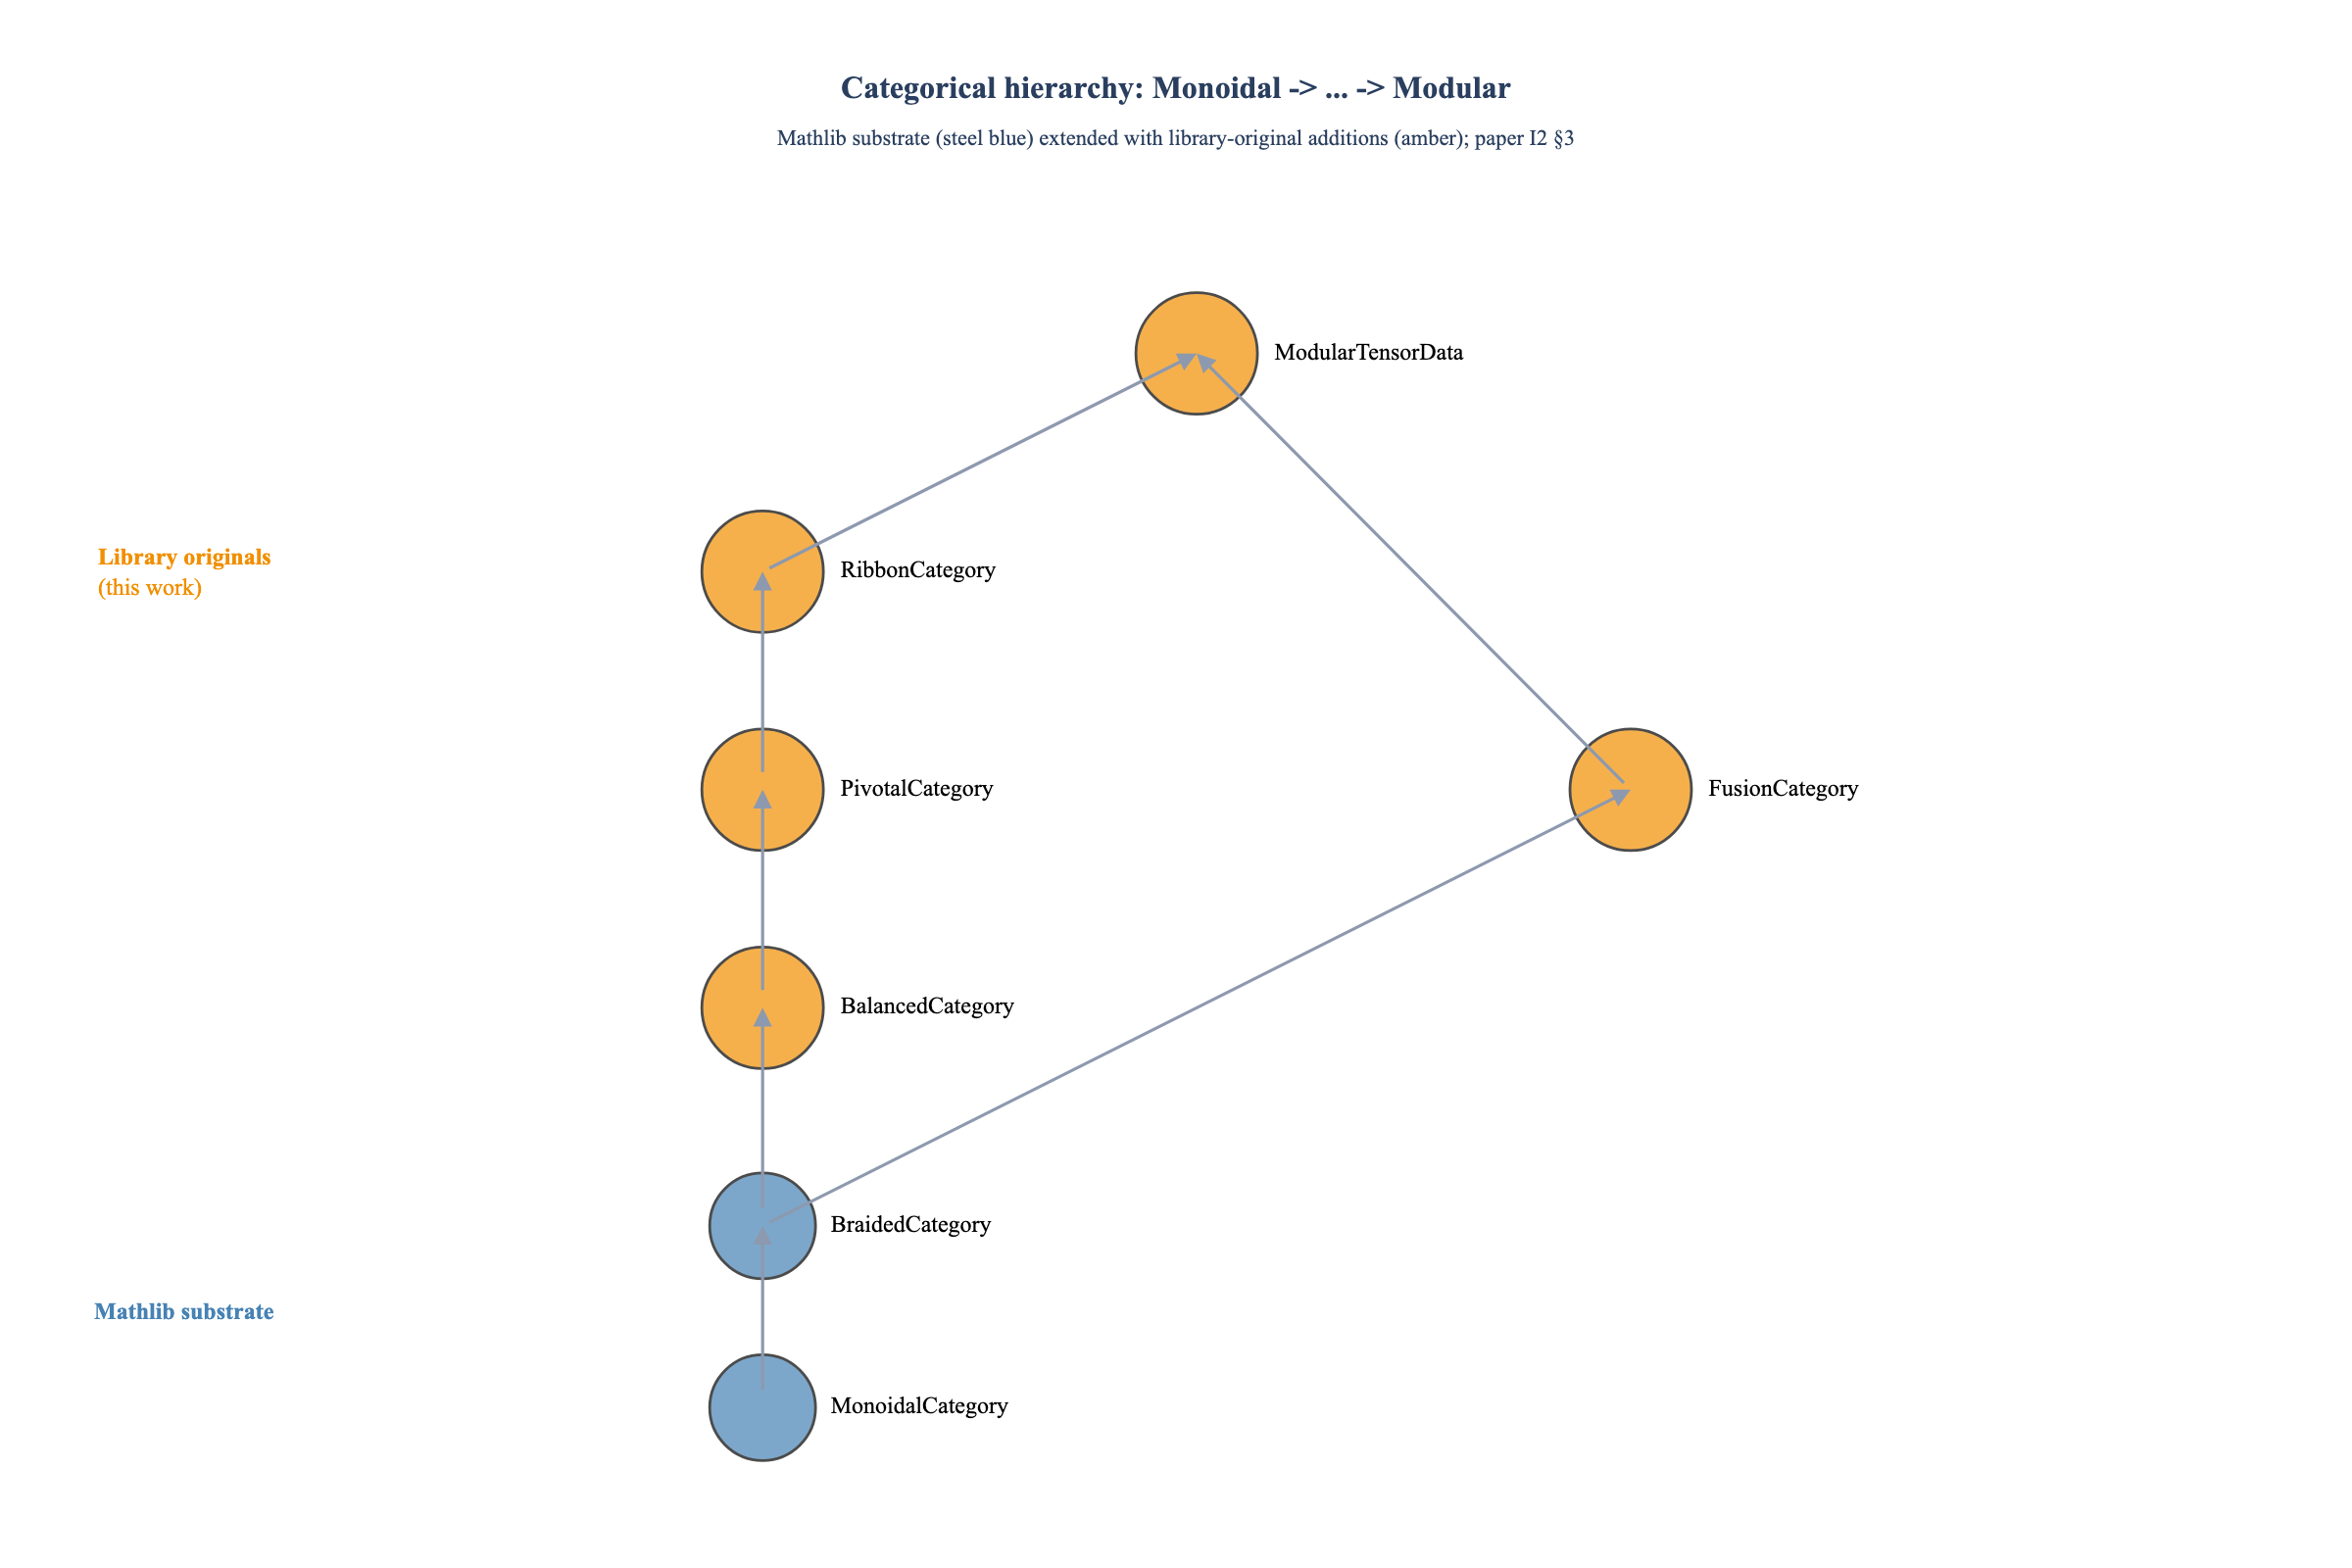
\includegraphics[width=0.75\linewidth]{figures/i2_fig1_categorical_hierarchy.png}
\caption{Categorical hierarchy as a Hasse-diagram poset. Mathlib's
existing \texttt{MonoidalCategory} and \texttt{BraidedCategory} (steel
blue, lower) provide the substrate. The library-original additions
\texttt{BalancedCategory}, \texttt{PivotalCategory},
\texttt{RibbonCategory}, and \texttt{FusionCategory} (amber) extend
the braided layer along two routes that converge in
\texttt{ModularTensorData}: one through the
balanced$\to$pivotal$\to$ribbon chain in
\texttt{RibbonCategory.lean}, and one through fusion (finite
semisimplicity) in \texttt{FusionCategory.lean}. An MTC is a fusion
category with ribbon structure satisfying the non-degeneracy
condition $\det S \neq 0$.}
\label{fig:i2-categorical-hierarchy}
\end{figure}

\subsection{Ribbon and modular tensor categories}

\texttt{RibbonCategory.lean} introduces three load-bearing
declarations:

\begin{itemize}
\item \texttt{class BalancedCategory} --- a braided monoidal
category equipped with a twist
$\theta : \mathbf{1} \Rightarrow \mathbf{1}$ satisfying the
balancing axiom
$\theta_{X \otimes Y} = (\theta_X \otimes \theta_Y) \circ
\beta_{Y, X} \circ \beta_{X, Y}$.
\item \texttt{class RibbonCategory} (extending
\texttt{BalancedCategory}, with \texttt{RigidCategory} as a
typeclass parameter) --- a balanced rigid category with the
twist--dual compatibility $\theta_{X^*} = (\theta_X)^*$. The class
hierarchy carries duals through the \texttt{RigidCategory}
parameter rather than via \texttt{PivotalCategory} inheritance; a
refactor to align with the textbook ``balanced + pivotal''
presentation of Bakalov--Kirillov / EGNO is a separate planned task.
\item \texttt{structure ModularTensorData} --- the structural data
for an MTC: a finite set of simple objects, an $S$-matrix, a
$T$-matrix (the twist read on the simple-object basis), and the
non-degeneracy condition $\det S \neq 0$ that promotes a fusion
category to a modular tensor category.
\end{itemize}

\texttt{BalancedCategory}, \texttt{RibbonCategory}, and
\texttt{ModularTensorData} are introduced here as Lean~4
typeclasses and structures suitable for downstream consumers in
topological-quantum-computation formalization.

\subsection{Spherical and pivotal structure}

\texttt{SphericalCategory.lean} (22 declarations including
18 theorems) builds the pivotal structure
$\mathrm{ev}_X^L : X^* \otimes X \to \mathbf{1}$ and
$\mathrm{coev}_X^L : \mathbf{1} \to X \otimes X^*$ together with
their right-handed duals, the snake equations, and the spherical
condition (left and right dimensions agree). The dimension function
$\dim_L X = \mathrm{tr}_L(\mathrm{id}_X)$ that downstream MTC
machinery depends on is defined here.

\subsection{Fusion structure}

\texttt{FusionCategory.lean} (20 declarations including 14 theorems)
encodes finite semisimplicity: a finite set of isomorphism classes
of simple objects, a unique simple unit, and the assertion that
every object is a finite direct sum of simples. The fusion
multiplicities $N_{XY}^Z$ satisfy associativity through the
6-$j$ symbols (encoded separately in module-specific F-symbol
files; see Section~\ref{sec:instances}).

%% ─────────────────────────────────────────────────────────────────
%% §4 Hopf algebra extensions
%% ─────────────────────────────────────────────────────────────────

\section{Hopf-Algebra Extensions and Quantum Groups}
\label{sec:hopf}

The library extends Mathlib's \texttt{HopfAlgebra} typeclass with
three quantum-group instances and two structural extensions
(quasitriangularity and the ribbon Hopf-algebra structure). Total
yield across four files: 114 declarations.

\subsection{$U_q(\mathfrak{sl}_2)$}

\texttt{Uqsl2Hopf.lean} (28 declarations) ships a Lean~4
formalization of the $U_q(\mathfrak{sl}_2)$ Hopf algebra. The algebra
generators $E$, $F$, $K$, $K^{-1}$ are encoded via Mathlib's
\texttt{RingQuot} construction on the free algebra modulo the
$U_q(\mathfrak{sl}_2)$ relations. The Hopf-algebra structure is
defined component-wise: coproduct
$\Delta(K) = K \otimes K$, $\Delta(E) = E \otimes K + 1 \otimes E$,
$\Delta(F) = F \otimes 1 + K^{-1} \otimes F$; counit
$\varepsilon(K) = 1$, $\varepsilon(E) = \varepsilon(F) = 0$;
antipode $S(K) = K^{-1}$, $S(E) = -EK^{-1}$, $S(F) = -KF$. The
file proves the four Hopf axioms (counit-coproduct compatibility,
antipode--multiplication compatibility, antipode--counit
compatibility, and coassociativity) component-wise on the
generators and lifts to the full algebra by induction on the
\texttt{RingQuot} construction.

The library exposes $U_q(\mathfrak{sl}_2)$ in two concrete
specializations: $q = 1$ (the classical limit, where the Hopf
structure reduces to the universal-enveloping-algebra Hopf
structure on $\mathfrak{sl}_2$) and a generic transcendental $q$
suitable for the $\mathrm{SU}(2)_k$ fusion category (with
$q = e^{i\pi/(k+2)}$).

\subsection{$U_q(\widehat{\mathfrak{sl}}_2)$}

\texttt{Uqsl2AffineHopf.lean} (25 declarations) extends the
construction to the affine quantum group, with central element $c$
and loop generators.

\subsection{$U_q(\mathfrak{sl}_3)$}

\texttt{Uqsl3Hopf.lean} (40 declarations) ships the rank-2 case. The
generators are $E_1, E_2, F_1, F_2, K_1, K_2$ and their inverses;
the relations include the quantum Serre relations
$E_1^2 E_2 - [2]_q E_1 E_2 E_1 + E_2 E_1^2 = 0$
(and the analogous $F$ relation).

\subsection{Structural extensions: Quasitriangular bialgebras and
Ribbon Hopf algebras}

\texttt{QuantumGroupHopf.lean} (21 declarations) defines the generic
quantum-group Hopf-algebra interface and structural lemmas. The
project's planned upstream PR-3 (Section~\ref{sec:upstream}) will
extract a typeclass \texttt{QuasitriangularBialgebra} (a Hopf
algebra equipped with an $R$-matrix satisfying the Yang--Baxter
and quasi-cocommutativity axioms) and a typeclass
\texttt{RibbonHopfAlgebra} (extending
\texttt{QuasitriangularBialgebra} with a central ribbon element
compatible with the antipode and the $R$-matrix). The Mathlib
PR will be accompanied by an instance proving that
$U_q(\mathfrak{sl}_2)$ satisfies
\texttt{QuasitriangularBialgebra} with the explicit $R$-matrix
$R = q^{H \otimes H/2} \sum_{n \geq 0} \frac{(q - q^{-1})^n}{[n]_q!}
q^{n(n-1)/2} (E^n \otimes F^n)$ in the universal closure. The
project-internal version of this content lives within
\texttt{QuantumGroupHopf.lean} as supporting lemmas; the
typeclass extraction is the upstream-PR target rather than a
shipped project artifact.

%% ─────────────────────────────────────────────────────────────────
%% §5 Decidable algebraic number fields
%% ─────────────────────────────────────────────────────────────────

\section{Decidable Algebraic Number Fields}
\label{sec:numberfields}

The categorical instances above need explicit field structure for
the eigenvalue and dimension computations
($d = \frac{1+\sqrt{5}}{2}$ for the Fibonacci anyon's quantum
dimension; $\zeta_{16}$ for the $\mathbb{Z}_{16}$-graded
$\mathrm{SU}(2)_4$ Verlinde ring; $\zeta_5$ for Fibonacci's
$T$-matrix). Mathlib's \texttt{NumberField} and
\texttt{IsCyclotomicExtension} are abstract; the library needed
\emph{decidable} arithmetic on these fields to support
\texttt{decide} and \texttt{native\_decide} tactics in the
fusion-instance proofs. We built nine decidable algebraic-number-field
modules.

\subsection{The $\mathbb{Q}(\sqrt{n})$ family}

\texttt{QSqrt2.lean} (18 declarations including 4 theorems),
\texttt{QSqrt3.lean} (26 declarations), and \texttt{QSqrt5.lean}
(20 declarations) implement the quadratic-extension fields with
explicit decidable equality. \texttt{QSqrt2} additionally exposes
decidable-arithmetic primitives that allow downstream code to use
\texttt{decide}-blocked equality on
$\mathbb{Q}(\sqrt{2})$-coefficient $S$-matrix entries without
opening Mathlib's abstract \texttt{AdjoinRoot} API. The planned
\texttt{ComputableAdjoinRoot}-style bridge between these two
representations --- not yet shipped as a separate file but
implicit in \texttt{QSqrt2.lean}'s structure --- is the leading
proposed Mathlib upstream PR (Section~\ref{sec:upstream}).

\subsection{The cyclotomic family}

\texttt{QCyc3.lean} (14), \texttt{QCyc5.lean} (35),
\texttt{QCyc5Ext.lean} (42), \texttt{QCyc15.lean} (21),
\texttt{QCyc15SqrtPhi.lean} (13), and \texttt{QCyc16.lean} (18)
implement the cyclotomic extensions $\mathbb{Q}(\zeta_n)$ for the
specific $n$ values needed by the project's MTC instances:
$\zeta_3$ for $\mathrm{SU}(3)_k=2$ centre, $\zeta_5$ for the
Fibonacci anyon, $\zeta_{15}$ for the
$\mathrm{SU}(2)_3 \times \mathrm{SU}(3)_1$ product, and
$\zeta_{16}$ for the project's $\mathbb{Z}_{16}$ anomaly
classification. \texttt{QCyc5Ext.lean} extends $\mathbb{Q}(\zeta_5)$
by $\sqrt{\varphi}$ (with $\varphi = (1 + \sqrt{5})/2$ the golden
ratio), the smallest extension in which Fibonacci's
$T$-matrix can be diagonalized over a single field with decidable
arithmetic.

The cumulative count is 207 declarations across the nine
algebraic-number-field modules. The decidability structure
integrates decidable-cyclotomic and decidable-quadratic-extension
arithmetic in a single library --- Mathlib provides each
separately, but supporting both $\sqrt{n}$ and $\zeta_n$ in the
same library with composable decidable equality is original to
this library.

%% ─────────────────────────────────────────────────────────────────
%% §6 Concrete MTC instances
%% ─────────────────────────────────────────────────────────────────

\section{Concrete Modular-Tensor-Category Instances}
\label{sec:instances}

The instances are organized by anyon family. Total yield across
ten files: 295 declarations.

\begin{figure}[h]
\centering
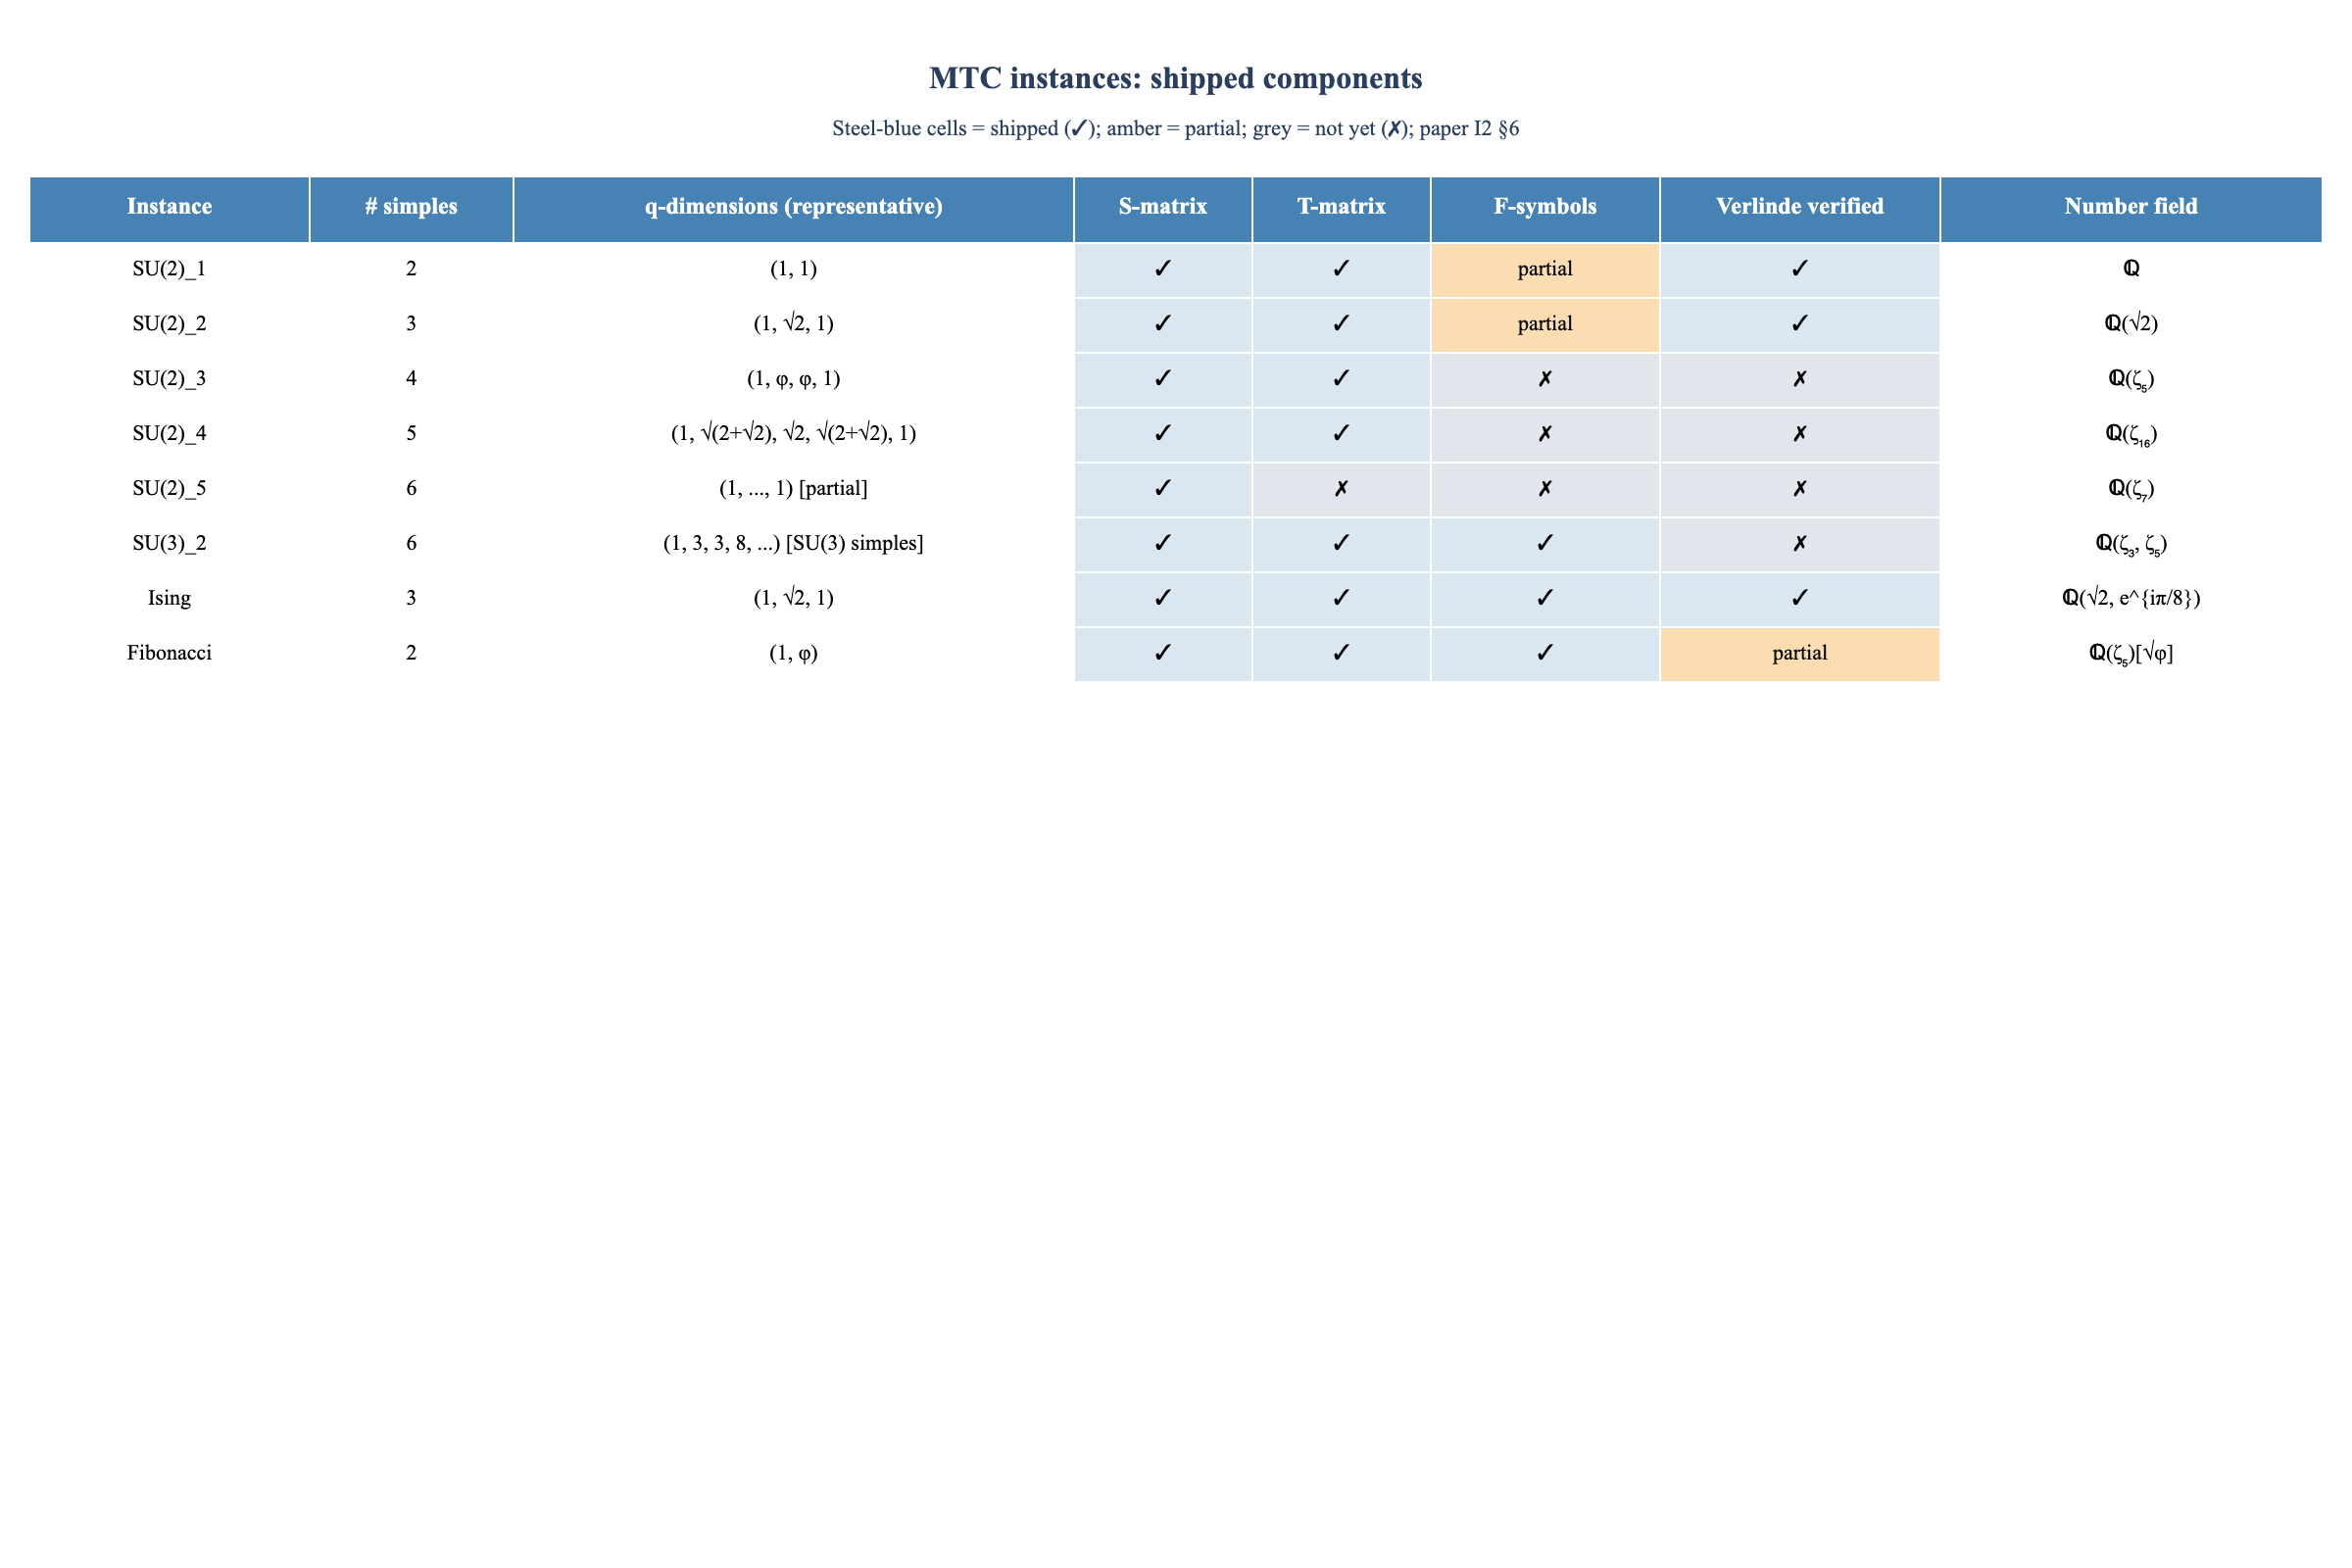
\includegraphics[width=0.95\linewidth]{figures/i2_fig3_mtc_instances.png}
\caption{Shipped-component status across the eight concrete
modular-tensor-category instances in the library:
$\mathrm{SU}(2)_{k}$ for $k = 1, \ldots, 5$, $\mathrm{SU}(3)_2$, the
Ising MTC, and the Fibonacci MTC. Columns track simple-object count,
representative quantum dimensions, and which of the
$S$-matrix, $T$-matrix, $F$-symbols, and Verlinde-formula are
formalized; the final column lists the underlying decidable algebraic
number field (Section~\ref{sec:numberfields}). Steel-blue cells mark
shipped components ($\checkmark$); amber, partial; cool grey, not yet
formalized.}
\label{fig:i2-mtc-instances}
\end{figure}

\subsection{$\mathrm{SU}(2)_k$ at $k = 1, \ldots, 5$}

\texttt{SU2kFusion.lean} (47 declarations including 46 theorems) is
the centerpiece. The fusion rules are encoded via a universal
truncated Clebsch--Gordan rule: for $0 \leq j_1, j_2 \leq k/2$,
\[
N_{j_1 j_2}^{j_3} = \begin{cases} 1 & \text{if } |j_1 - j_2| \leq j_3
\leq \min(j_1 + j_2, k - j_1 - j_2), \; j_1 + j_2 + j_3 \in
\mathbb{Z} \\ 0 & \text{otherwise.} \end{cases}
\]
The file proves fusion associativity at every $k = 1, 2, 3, 4, 5$
by \texttt{decide}, leveraging the decidable-arithmetic
infrastructure of Section~\ref{sec:numberfields}. The library
computes the $\mathrm{SU}(2)_k$ MTC fusion rule \emph{from} the
$U_q(\mathfrak{sl}_2)$ quantum-group structure of
Section~\ref{sec:hopf} rather than postulating it as a separate
combinatorial datum.

\texttt{SU2kMTC.lean} (17 declarations) instantiates
\texttt{ModularTensorData} for each $k$. \texttt{SU2kSMatrix.lean}
(20 declarations) computes the explicit $S$-matrix
$S_{j_1 j_2} = \sqrt{\frac{2}{k+2}}
\sin\!\frac{(2j_1+1)(2j_2+1)\pi}{k+2}$ and proves the Verlinde
formula
$N_{j_1 j_2}^{j_3} = \sum_{j} \frac{S_{j_1 j} S_{j_2 j}
\overline{S_{j_3 j}}}{S_{0 j}}$ for the cases $k = 1$ and $k = 2$
(theorems \texttt{verlinde\_k1\_11\_0}, \texttt{verlinde\_k1\_11\_1},
\texttt{verlinde\_k2\_sigma\_sq\_vacuum},
\texttt{verlinde\_k2\_sigma\_sq\_no\_sigma},
\texttt{verlinde\_k2\_sigma\_sq\_psi},
\texttt{verlinde\_k2\_psi\_sq\_vacuum}); Verlinde-formula
verification at $k = 3, 4, 5$ is not yet shipped (the fusion
associativity at those levels is proven separately in
\texttt{SU2kFusion.lean}).

\subsection{$\mathrm{SU}(3)_k$ at $k = 1, 2$}

\texttt{SU3kFusion.lean} (29 declarations) ships the rank-2 fusion
rules. \texttt{SU3k2SMatrix.lean} (27 declarations) and
\texttt{SU3k2FSymbols.lean} (12 declarations) ship the
$\mathrm{SU}(3)_k=2$ specialization, including the F-matrix on the
Fibonacci sub-block (the $F^2 = I$ involution is proven; the full
$120$-entry F-symbol catalog and the full hexagon and pentagon
equation discharges are deferred per the module's docstring) and
the explicit $T$-matrix diagonalizable over
$\mathbb{Q}(\zeta_3, \zeta_5)$.

\subsection{Ising MTC}

\texttt{IsingBraiding.lean} (34 declarations including 24 theorems)
ships the Ising MTC (central charge $c = 1/2$): the three simple
objects $\{\mathbf{1}, \sigma, \psi\}$, the fusion rules
$\sigma \otimes \sigma = \mathbf{1} \oplus \psi$,
$\psi \otimes \psi = \mathbf{1}$, and the $R$-matrices
$R^{\sigma \sigma}_{\mathbf{1}} = e^{i\pi/8}$,
$R^{\sigma \sigma}_\psi = e^{-3i\pi/8}$ that encode the
Majorana-fermion braiding. \texttt{IsingGates.lean} (36
declarations) is the topological-quantum-computation sidebar:
explicit braid matrices that implement the Clifford gates by
$\sigma$-anyon braiding.

\subsection{Fibonacci MTC}

\texttt{FibonacciBraiding.lean} (55 declarations including 32
theorems) is the largest single instance file in the library. The
two simple objects are $\mathbf{1}$ and $\tau$ (the Fibonacci
anyon, with quantum dimension $d_\tau = \varphi$). The fusion rule
$\tau \otimes \tau = \mathbf{1} \oplus \tau$ is the source of the
Fibonacci recurrence (number of fusion outcomes for $n$ copies of
$\tau$). The R-matrices and F-symbols are computed in
$\mathbb{Q}(\zeta_5)[\sqrt{\varphi}]$ via the
\texttt{QCyc5Ext.lean} infrastructure of
Section~\ref{sec:numberfields}. \texttt{FibonacciMTC.lean}
(18 declarations) wraps the result as a \texttt{ModularTensorData}
instance and proves the pentagon identity (theorem
\texttt{fib\_pentagon}, line~106) by \texttt{native\_decide} on the
512-case F-symbol catalog. The hexagon identity is not yet shipped
as a named theorem in either Fibonacci file.

%% ─────────────────────────────────────────────────────────────────
%% §7 Mathlib upstream coordination
%% ─────────────────────────────────────────────────────────────────

\section{Mathlib Upstream Coordination Plan}
\label{sec:upstream}

The library is currently vendored within the SK--EFT Hawking
project as
\texttt{lean/SKEFTHawking/\{KLinearCategory, FusionCategory, ...\}}
and mirrored in the open-source extraction repository
\texttt{NetRxn/lean-tensor-categories} as a standalone Lake project
under Apache~2.0. The mid-term plan is to upstream the
content into Mathlib through a sequence of atomic pull requests.
This section documents the plan for transparency.

\begin{figure}[h]
\centering
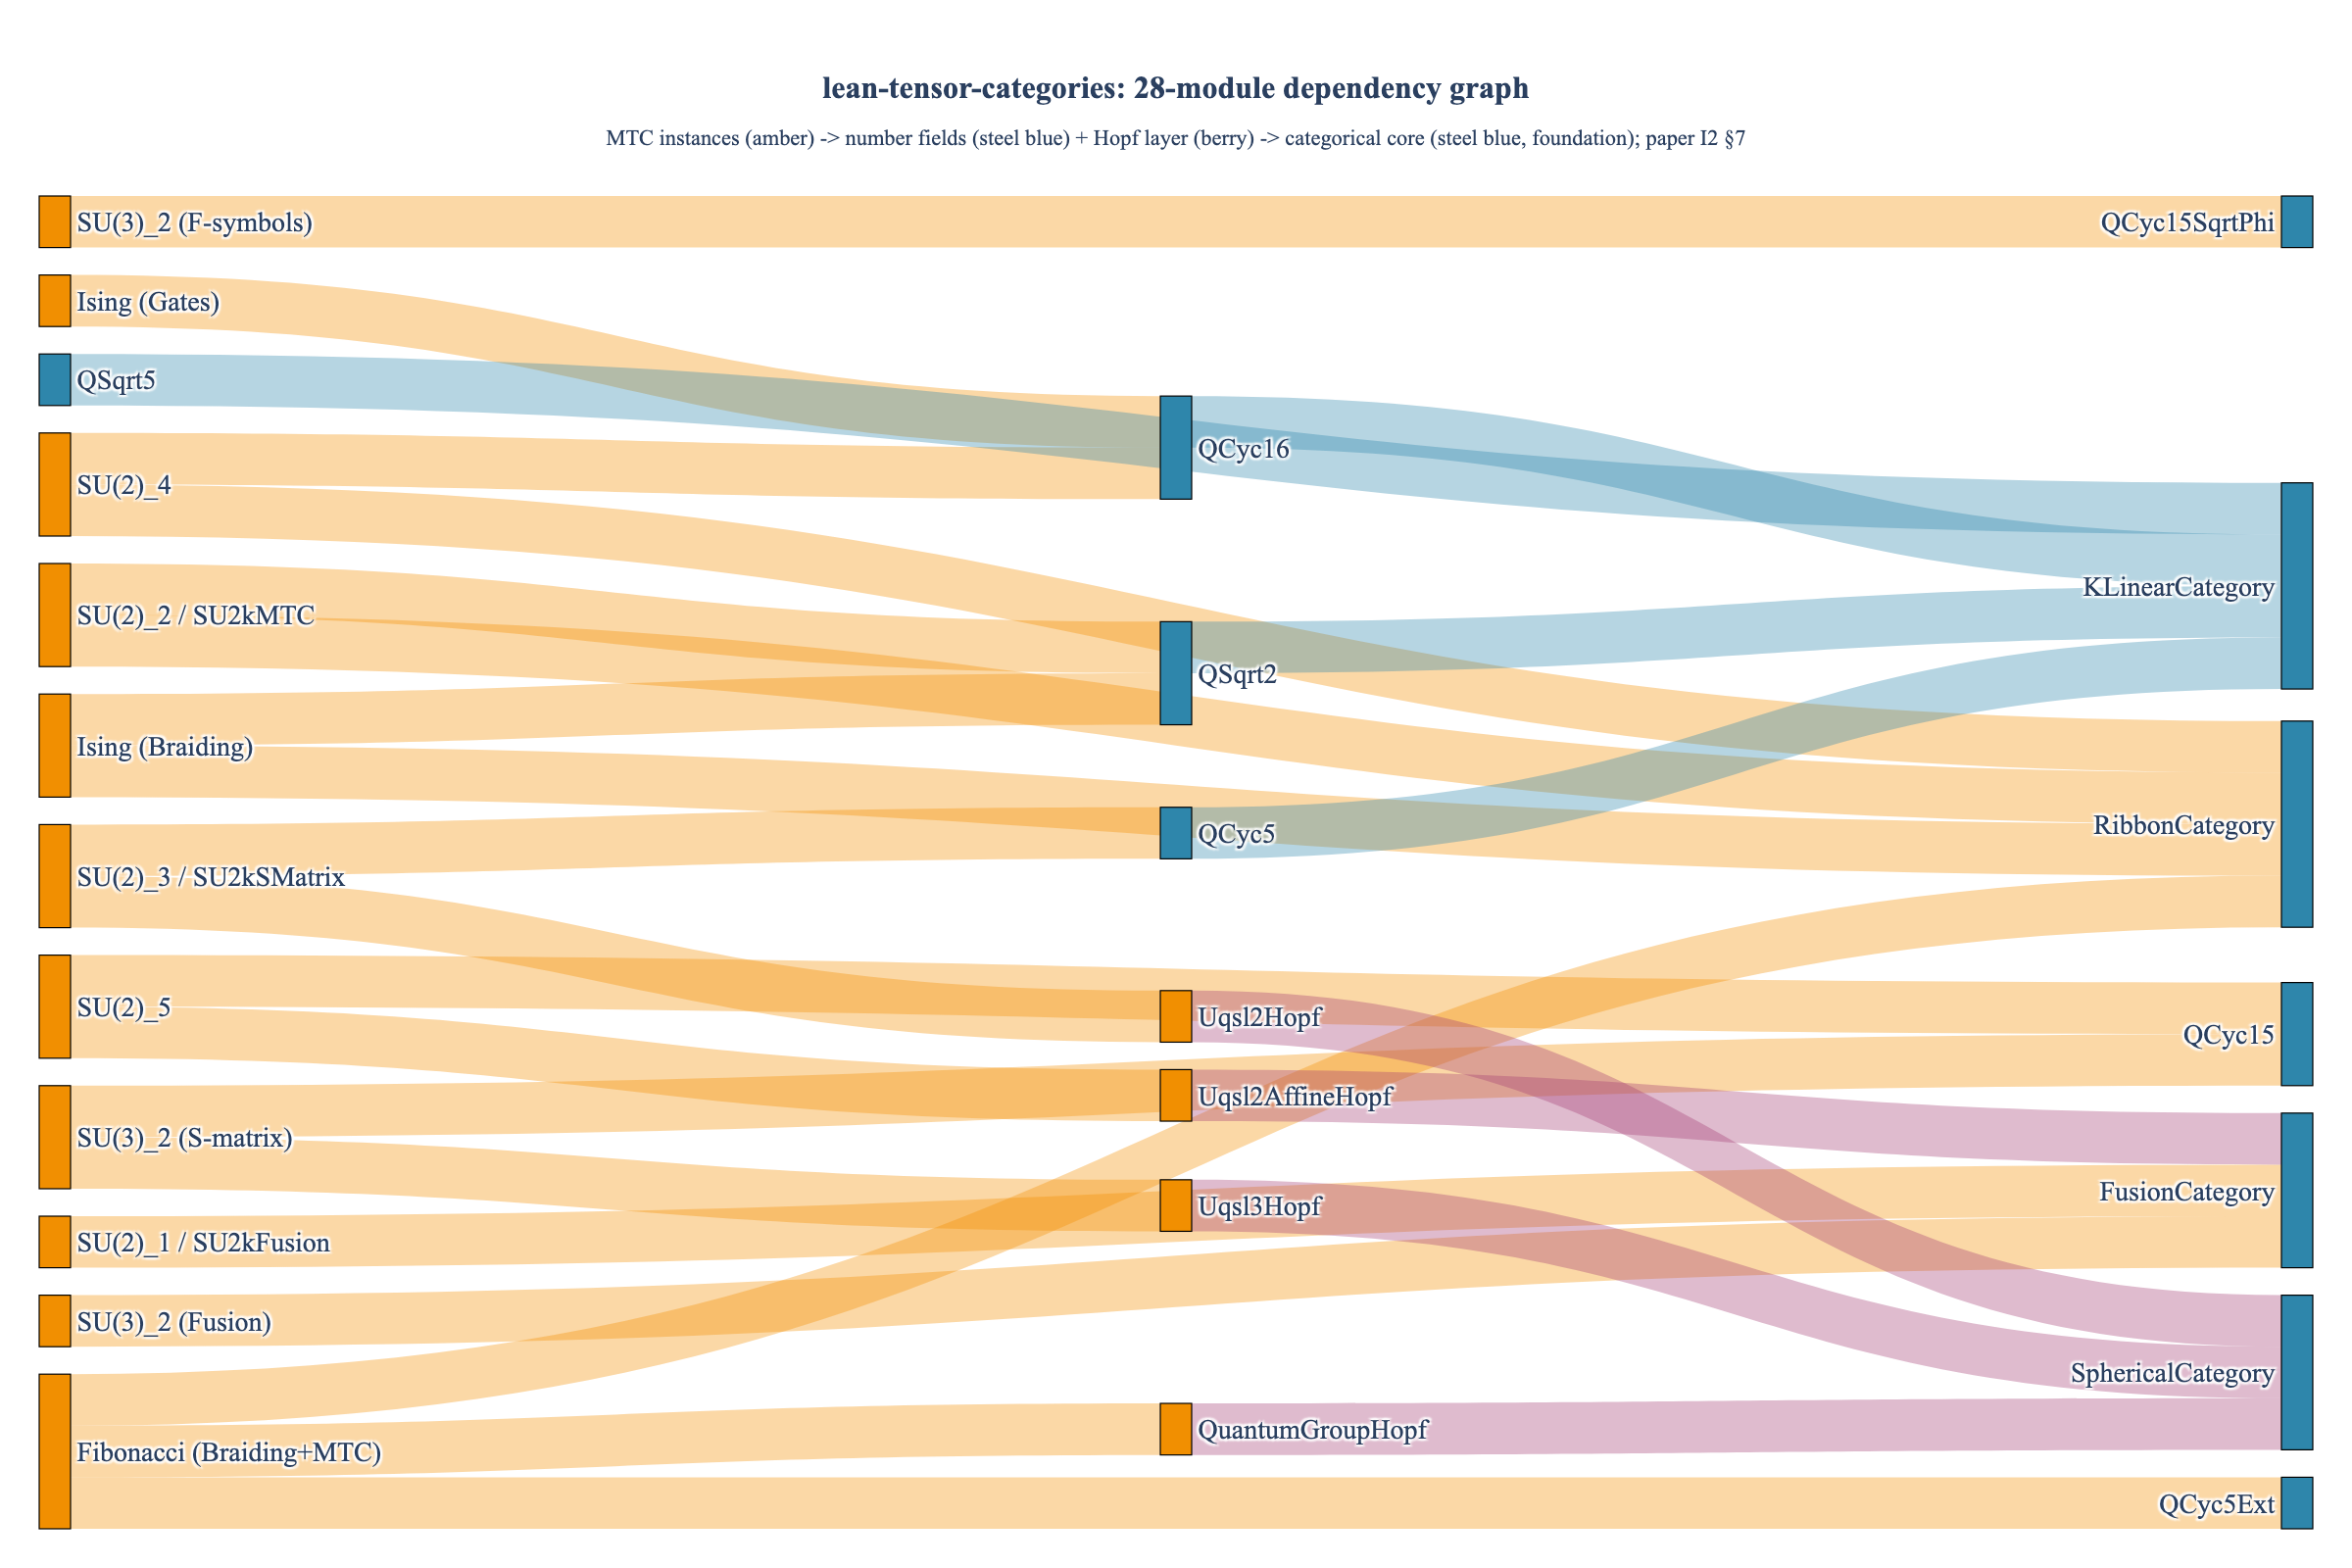
\includegraphics[width=0.95\linewidth]{figures/i2_fig2_module_dependencies.png}
\caption{Dependency graph of the 27 modules that comprise the
\texttt{lean-tensor-categories} library, organized into four
architectural tiers: the categorical core (steel blue;
Section~\ref{sec:categorical}), the Hopf-algebra layer (berry;
Section~\ref{sec:hopf}), the decidable-algebraic-number-field family
(steel blue, mid; Section~\ref{sec:numberfields}), and the ten
concrete MTC-instance modules (amber; Section~\ref{sec:instances};
the table-figure of Section~\ref{sec:instances} surveys the eight
distinct anyon families covered by these ten files). Sankey
flows go from each instance through the number-field and Hopf layers
to the categorical foundation, illustrating how the layered
architecture lets each MTC instance be expressed as a thin
specialization of the substrate.}
\label{fig:i2-module-deps}
\end{figure}

\subsection{Relationship-building gate}

Before any pull request is filed, three relationship-building
conditions must be met:

\begin{itemize}
\item \textbf{R1: Mathlib Zulip introduction.} A formal
introduction in Mathlib's Zulip
\texttt{\#mathlib4 > new contributors} stream and
\texttt{\#mathlib4 > maths > category theory} stream describing
the project, the proposed scope, and the invitation to discussion.
\item \textbf{R2: AI-tool-assistance disclosure.} Transparent
disclosure that Lean theorems in the proposed library were
generated with ``substantive AI-tool assistance under human
direction'' (the project's standard attribution language). The
disclosure invites discussion on attribution, review protocols,
and acceptance policy. The library's
\texttt{ATTRIBUTION.md} file in the extraction repo carries the
attribution language that the discussion will reference.
\item \textbf{R3: PR-strategy discussion.} Agreed sub-PR
sequencing with the relevant Mathlib maintainers (currently the
category-theory and number-theory maintainers; AlgebraicGeometry
maintainers may join the discussion when the cyclotomic content
is reached).
\end{itemize}

\subsection{Atomic-PR sequence}

The proposed sequence is:

\begin{enumerate}
\item \textbf{PR-1: \texttt{QSqrt2 + ComputableAdjoinRoot bridge}.}
The narrowest, highest-utility PR. Adds a decidable-arithmetic
bridge to \texttt{Mathlib.NumberTheory.QuadraticField.Basic}.
Self-contained, broad utility (number theory, algebraic geometry).
\item \textbf{PR-2: \texttt{PivotalCategory}, \texttt{RibbonCategory}.}
New files under \texttt{Mathlib.CategoryTheory.Monoidal}; extends
existing \texttt{MonoidalCategory} and \texttt{BraidedCategory}.
\item \textbf{PR-3: \texttt{QuasitriangularBialgebra},
\texttt{RibbonHopfAlgebra}.} New file under
\texttt{Mathlib.RingTheory.HopfAlgebra}; extends Mathlib's
existing \texttt{HopfAlgebra} typeclass.
\item \textbf{PR-4+: MTC instances.} \texttt{Ising}, Fibonacci,
$\mathrm{SU}(2)_k$. Lower priority; may stay project-local at
maintainer discretion.
\end{enumerate}

\subsection{The AI-tool-assistance disclosure protocol}

Mathlib's contribution policy on AI-generated content was, as of
2026-04-30, in flux. The protocol the project operates under is:
(i)~every PR description discloses ``drafted with AI-tool assistance
under human review and direction''; (ii)~every theorem in the
library has been re-read by a human contributor before commit;
(iii)~every PR is accompanied by a separate cover memo in the
relevant Zulip thread describing which subsystems received the
heaviest assistance and the human-review protocol applied to them.
The protocol is not a request for special treatment; it is
disclosure that lets reviewers calibrate effort. We expect Mathlib's
acceptance threshold to be the same for AI-assisted contributions
as for unassisted ones --- the standard is correctness, mathematical
relevance, and engineering quality, not the provenance of the
typing.

\begin{figure}[h]
\centering
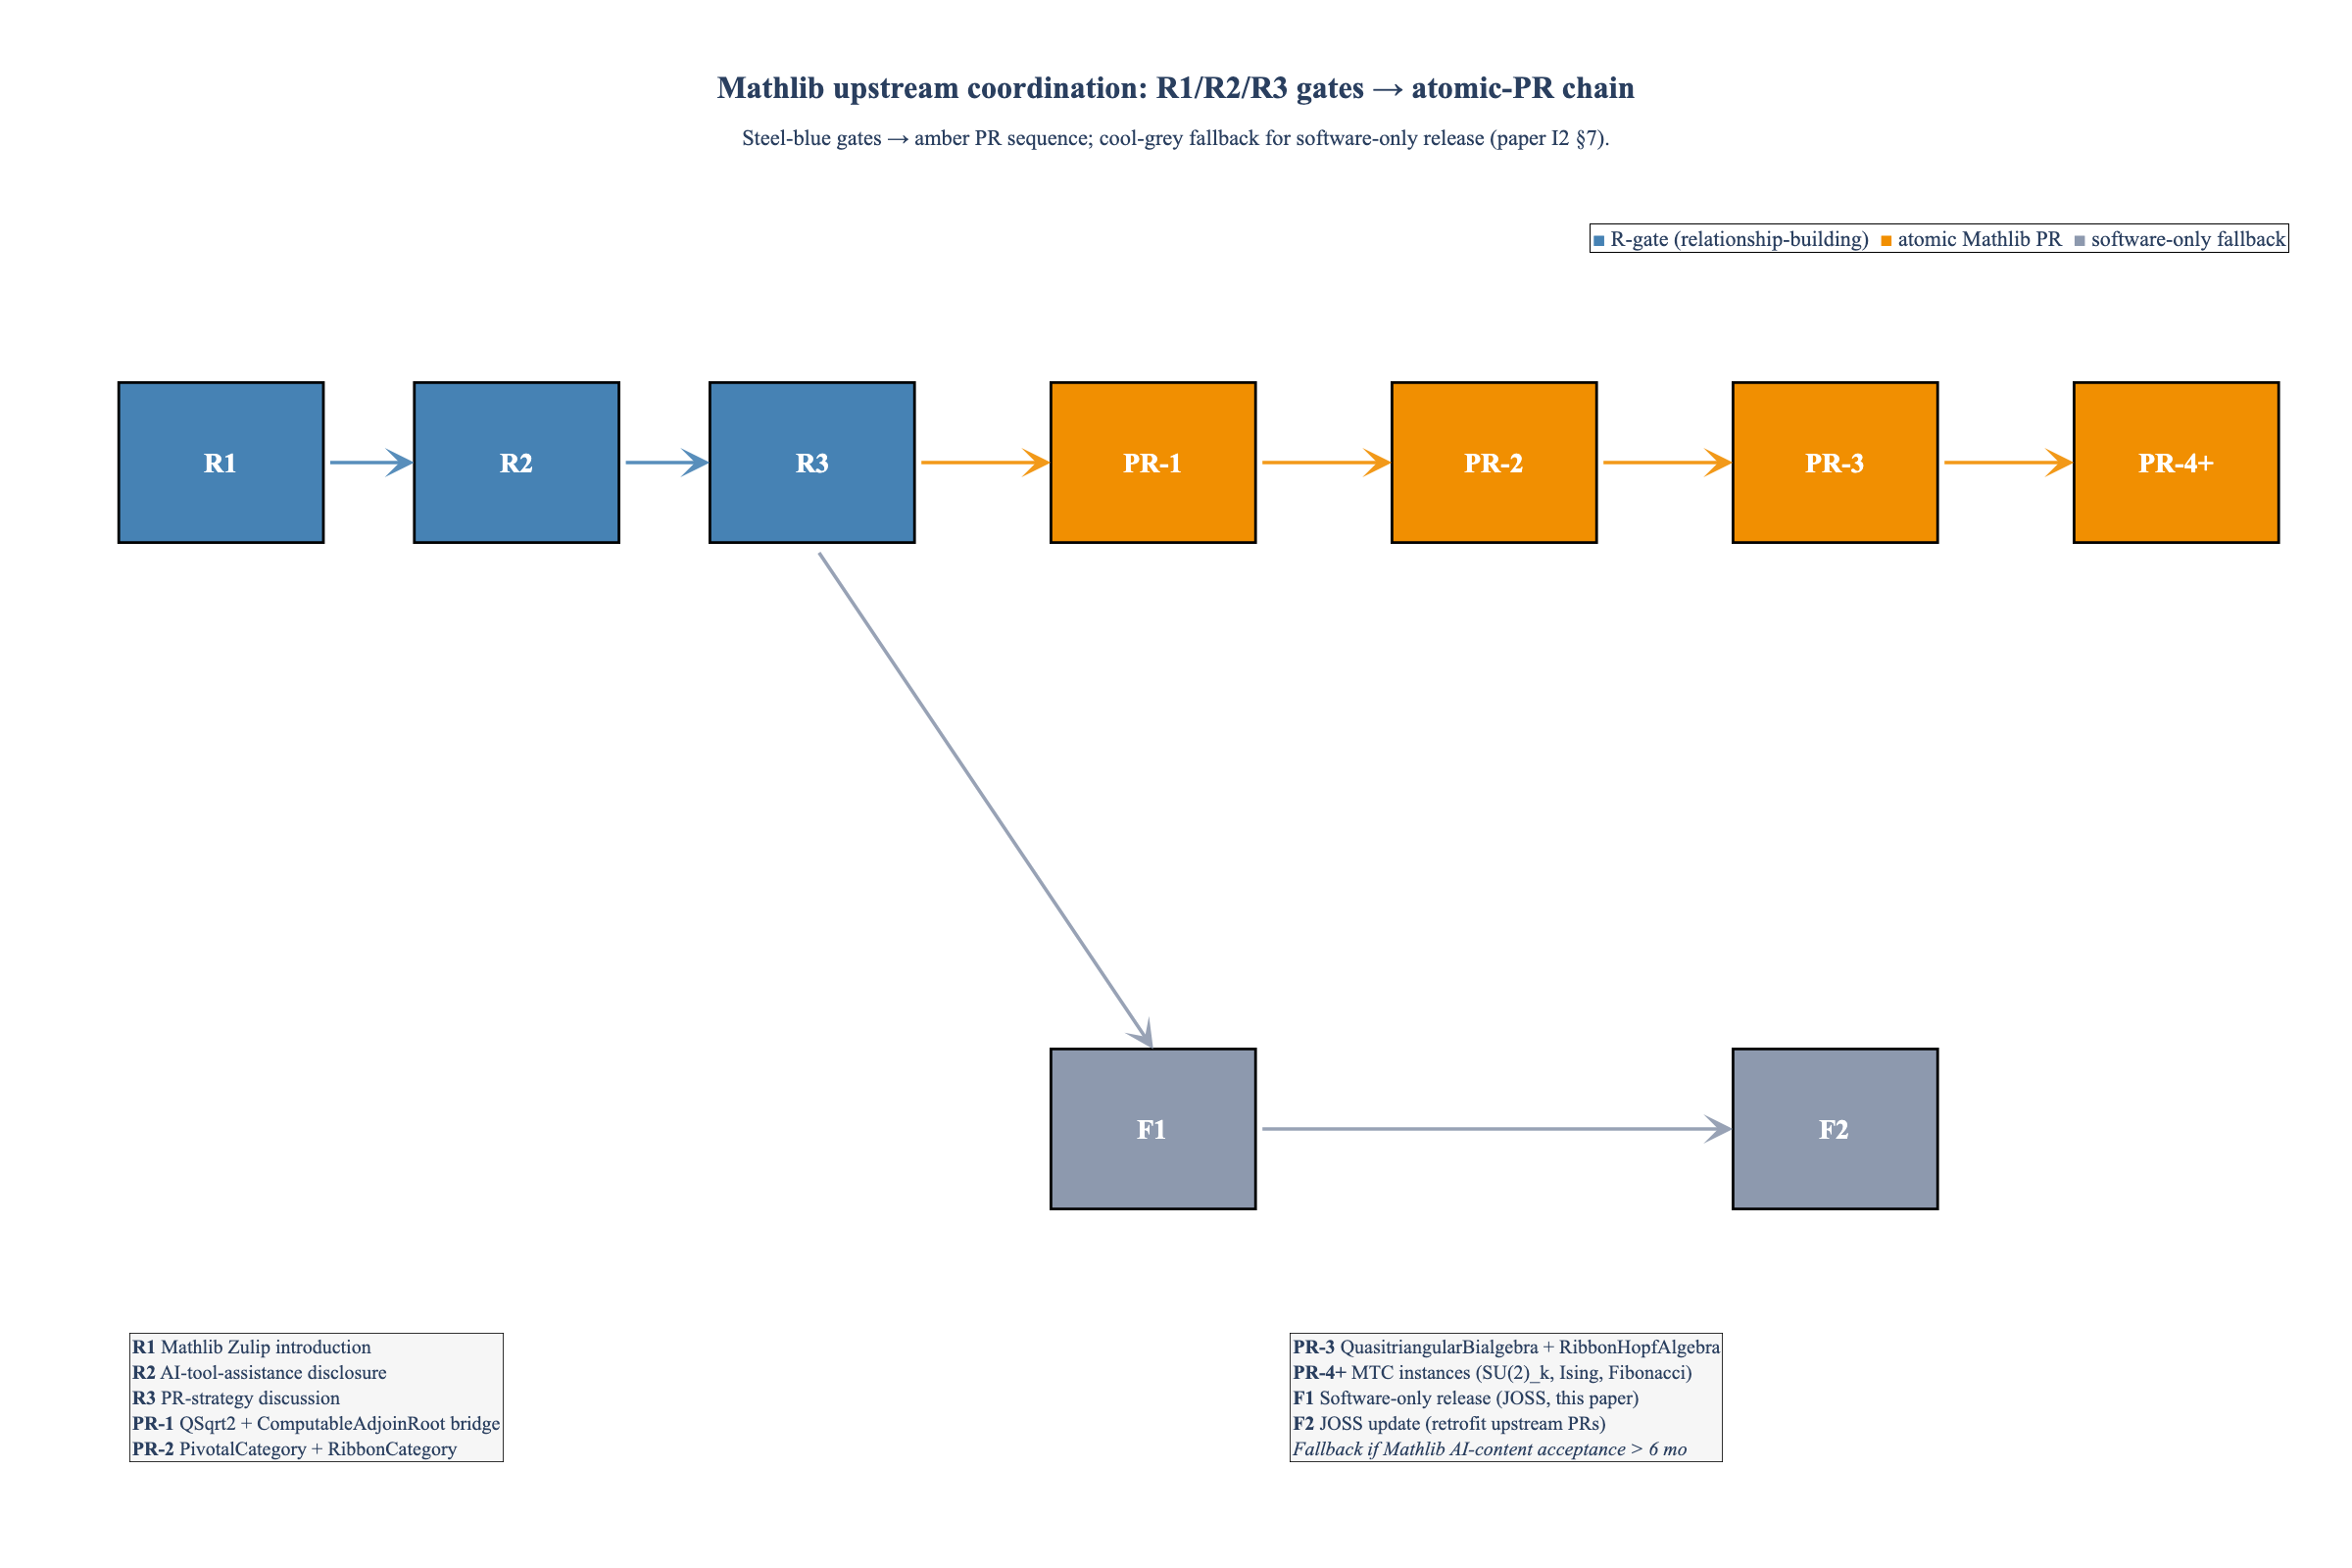
\includegraphics[width=0.95\linewidth]{figures/i2_fig5_mathlib_upstream_flow.png}
\caption{Mathlib upstream coordination flow. Three sequential
relationship-building gates --- R1 (Mathlib Zulip introduction),
R2 (AI-tool-assistance disclosure), R3 (PR-strategy discussion with
maintainers) --- precede the atomic-PR chain: PR-1 \texttt{QSqrt2 +
ComputableAdjoinRoot} bridge, PR-2 \texttt{PivotalCategory +
RibbonCategory}, PR-3 \texttt{QuasitriangularBialgebra +
RibbonHopfAlgebra}, and PR-4+ MTC instances. The cool-grey branch
shows the fallback path: if the gate is delayed beyond approximately
six months, the library ships as a software-only artifact through
this paper, with the Mathlib-acceptance hook handled later as a
separate JOSS-record update.}
\label{fig:i2-mathlib-upstream-flow}
\end{figure}

\subsection{Conditional path: software-only release}

If Mathlib's AI-content acceptance is delayed beyond approximately
six months (the I2 timeline window), the library ships as a
software-only artifact through this paper without the
Mathlib-acceptance hook. The upstream cycle becomes a separate
update to the JOSS record. The library's standalone Lake project
in \texttt{NetRxn/lean-tensor-categories} is structured to support
this fallback: the dependency on the SK--EFT Hawking codebase is
zero; the dependency on Mathlib is at a stable pinned commit; the
test suite and CI run independently.

%% ─────────────────────────────────────────────────────────────────
%% §8 Reusability and downstream applications
%% ─────────────────────────────────────────────────────────────────

\section{Reusability and Downstream Applications}
\label{sec:reusability}

The library was developed for the SK--EFT Hawking program but is
deliberately scoped for general reuse. The design choices that
support this:

\begin{itemize}
\item \textbf{Zero physics-specific imports.} The library does not
import \texttt{constants.py}, \texttt{formulas.py}, or any
SK--EFT Hawking module. Every theorem is a statement of mathematics,
not of substrate-emergent fluid dynamics.
\item \textbf{Mathlib-pinned, not Mathlib-dependent at HEAD.} The
\texttt{lean-toolchain} pin is on a fixed Mathlib commit, not on
\texttt{main}. Downstream consumers can pin the same commit
without inheriting the rest of SK--EFT Hawking's vendored stack.
\item \textbf{Decidable arithmetic is composable.} The
$\mathbb{Q}(\sqrt{n})$ and $\mathbb{Q}(\zeta_n)$ infrastructures
are designed to compose: a downstream consumer can extend
$\mathbb{Q}(\zeta_5)$ by $\sqrt{\varphi}$ in the same idiom as
$\mathbb{Q}$ extends to $\mathbb{Q}(\sqrt{2})$, and the resulting
\texttt{decide}-blocked tactics behave the same way.
\end{itemize}

The intended downstream applications include:

\begin{itemize}
\item \textbf{Topological-QFT formalization.} Anyon-Wilson-line
algebras, partition-function evaluations on closed 3-manifolds,
Reshetikhin--Turaev surgery formulas~\cite{turaev2010}. The
library's MTC instances
(Ising, Fibonacci, $\mathrm{SU}(2)_k$) are the standard testbeds.
\item \textbf{Fault-tolerant quantum-computing infrastructure.} The
Ising-anyon braid matrices in
\texttt{IsingGates.lean} match the structure of gates targeted by
non-Abelian-anyon topological-quantum-computing roadmaps in the
broader research community pursuing Majorana-fermion-based
non-Abelian-anyon platforms (including industrial proposals such
as Microsoft Quantum's and academic/national-lab
Majorana-detection experiments); the
Fibonacci universality infrastructure in
\texttt{FibonacciBraiding.lean} (R-matrix non-trivial-eigenvalue
checks, $\sigma$-matrix orders, density-of-image conditions) is
the formal substrate from which the textbook universality result
that motivates topological-QC research can be assembled. The
companion module \texttt{FibonacciUniversality.lean} formalizes
the Lie-algebra-spanning argument (compact-Lie-group iterated
commutators of $\sigma_1, \sigma_2$ spanning $\mathfrak{su}(2)$
imply dense generation of $\mathrm{SU}(2)$) following
Freedman--Larsen--Wang and Kuperberg; the explicit density
theorem (``the shipped iterated-commutator spanning condition
implies $\overline{\langle \sigma_1, \sigma_2 \rangle} = \mathrm{SU}(2)$'')
is not shipped as a single named theorem. A formally verified
gate compiler can build on the library without re-deriving the
categorical substrate.
\item \textbf{Lattice statistics.} \texttt{VerifiedJackknife} is
immediately usable by any lattice-Monte-Carlo project: the
estimators are deterministic functions on finite samples, so
adopting them in another physics codebase is a matter of importing
the module and verifying the lattice-style traversal helpers.
\item \textbf{Emergent-MTC black-hole-entropy formalization.} The
Kaul--Majumdar SU$(2)_k$ decomposition of the
Bekenstein--Hawking entropy can be formalized using
\texttt{SU2kMTC.lean} as the substrate; the
$-\frac{3}{2} \log(A/(4G_N))$ correction term is then a
consequence of the formal MTC structure modulo the
\texttt{IsolatedHorizonHypotheses} structure declared in
\texttt{lean/SKEFTHawking/RTReplicaTrickOnMTC.lean}, which
packages the loop-quantum-gravity isolated-horizon assumptions
explicitly (mean-curvature gauge, generator-vector-field gauge,
spin-network-basis admissibility) rather than treating them as
hidden inputs to the MTC calculation. The SK--EFT Hawking
program's emergent-gravity deep paper (bundle D3) documents the
full dependency.
\item \textbf{Anomaly classification.} The
$\mathbb{Z}_{16}$-graded structure on
$\mathrm{SU}(2)_4 \times \mathrm{SU}(2)_4$ is encoded via
\texttt{QCyc16.lean} and used in the project's anomaly-constraints
deep paper (D2 in the project's bundle architecture).
\end{itemize}

%% ─────────────────────────────────────────────────────────────────
%% §9 Discussion
%% ─────────────────────────────────────────────────────────────────

\section{Discussion: Related Work, Limitations, Future Extensions}
\label{sec:discussion}

\subsection{Related work}

Mathlib's existing categorical infrastructure
(\texttt{MonoidalCategory}, \texttt{BraidedCategory}, monoidal
functors) is the substrate this library extends. The Coq/Rocq
ecosystem has \texttt{UniMath}, an extensive univalent-foundations
library that includes monoidal and (some) bicategory infrastructure
but does not (as of our 2026 prior-art sweep) ship a non-trivial
Hopf algebra, a Ribbon Hopf algebra typeclass, or modular tensor
categories \emph{as such}; the Agda \texttt{categories} library
covers similar foundational categorical content with comparable
scope. The content shipped here that complements rather than
duplicates those ecosystems --- documented by the prior-art search
in the SK--EFT Hawking project's \texttt{Lit-Search/Phase-5o/}
dossier --- comprises: a non-trivial Hopf algebra in three
specializations ($U_q(\mathfrak{sl}_2)$,
$U_q(\widehat{\mathfrak{sl}}_2)$, $U_q(\mathfrak{sl}_3)$); the
Ribbon and Modular Tensor Category typeclasses; an MTC fusion-rule
instance computed from a quantum group ($\mathrm{SU}(2)_k$ and
$\mathrm{SU}(3)_k=2$); and a decidable algebraic-number-field bridge
supporting both $\sqrt{n}$ extensions and $\zeta_n$ in the same
library with composable decidable equality.

For verified statistical estimators, the closest prior work we
found is the lattice-QCD validation in the
\texttt{Math-Components} \texttt{ssreflect} ecosystem of basic
arithmetic identities used in lattice analysis; this does not
include the jackknife or autocorrelation estimators themselves.
Outside the proof-assistant world, the lattice-QCD community
operates on extensively-tested but unverified C++ implementations
(the SciDAC/USQCD Chroma codebase being a representative example
of unverified production lattice-QCD software);
\texttt{VerifiedJackknife} is an addition to that ecosystem, not
a replacement.

\subsection{Limitations}

The categorical library is at the structural-level scope:
typeclasses, instances on small examples, and the explicit fusion /
S-matrix / F-symbol computations. The library does not yet ship:

\begin{itemize}
\item \textbf{The Drinfeld center construction.} The library has
the prerequisite typeclass machinery to define
$\mathcal{Z}(\mathcal{C})$ but the construction is not in this
release. Phase 5q of the SK--EFT Hawking project shipped a
project-internal Drinfeld-center module; that module is targeted
for a follow-up extraction.
\item \textbf{The Reshetikhin--Turaev partition-function-on-3-manifolds
construction.} The MTC machinery is sufficient for it, but the
3-manifold-handle-decomposition substrate is itself a separate
infrastructure project that the SK--EFT Hawking program touches
only at the structural-Prop scoping level
(see SK--EFT Hawking paper~I1 §13 for the structural-Prop scoping
discipline).
\item \textbf{The probability-theory layer for
\texttt{VerifiedJackknife}.} Statements about unbiasedness or
asymptotic distributions require Mathlib's
\texttt{Probability.Statistics} layer at a scope that does not
yet exist; the library's claim is the deterministic structural
content only.
\end{itemize}

\subsection{Future extensions}

Three extensions are planned for subsequent development:

\begin{itemize}
\item \textbf{Drinfeld center.} The categorical-center construction
$\mathcal{Z}(\mathcal{C})$ for a finite tensor category
$\mathcal{C}$, with the modular-double universality theorem
$\mathcal{Z}(\mathcal{C})$ is modular when $\mathcal{C}$ is fusion.
\item \textbf{$\mathrm{SU}(2)_k$ at $k = 6, 7, 8$.} The current
library ships $k = 1, \ldots, 5$; extensions to higher levels
require additional cyclotomic-extension infrastructure that is
straightforwardly composable from the existing nine number-field
modules.
\item \textbf{The \texttt{LinearAlgebra.Eigenvalues.Concrete}
extension.} The library uses Mathlib's abstract eigenvalue API in
several places; a concrete-eigenvalue extension that supports
\texttt{decide}-blocked eigenvalue extraction over algebraic
number fields would simplify several
$\mathrm{SU}(2)_k$ S-matrix computations and is itself a
candidate Mathlib upstream PR.
\end{itemize}

The library is open-source, scoped for general reuse, and ready
for adoption by any Lean~4 project requiring verified
modular-tensor-category infrastructure, verified jackknife or
autocorrelation estimators, or the decidable algebraic-number-field
substrate that supports them.

%% ─────────────────────────────────────────────────────────────────

\begin{thebibliography}{99}
\bibitem{efron1982} B.~Efron, \emph{The Jackknife, the Bootstrap,
and Other Resampling Plans}, SIAM CBMS-NSF Regional Conference
Series in Applied Mathematics 38 (1982).
\bibitem{wolff2004} U.~Wolff, ``Monte Carlo
errors with less errors,''
\emph{Comput. Phys. Commun.}\ \textbf{156}, 143--153 (2004);
arXiv:hep-lat/0306017.
\bibitem{bakalov2001} B.~Bakalov and A.~Kirillov,
\emph{Lectures on Tensor Categories and Modular Functor},
American Mathematical Society University Lecture Series 21 (2001).
\bibitem{egno2015} P.~Etingof, S.~Gelaki, D.~Nikshych, and
V.~Ostrik, \emph{Tensor Categories}, AMS Mathematical Surveys and
Monographs 205 (2015).
\bibitem{turaev2010} V.~G.~Turaev, \emph{Quantum Invariants of Knots
and 3-Manifolds}, de Gruyter Studies in Mathematics 18 (de Gruyter,
2010 ed.).
\bibitem{kassel1995} C.~Kassel, \emph{Quantum Groups}, Springer
Graduate Texts in Mathematics 155 (1995).
\bibitem{mathlib4} The Mathlib Community, ``The Lean Mathematical
Library,'' \emph{Proc.\ CPP 2020} (2020); current pin in
SK--EFT Hawking's \texttt{lean/lakefile.toml}.
\end{thebibliography}


%% ─── Lifted from _phase6n_W1b_lean_only (§5) — 2026-05-06T15:43:01Z ───
%% \section{SymTFT audit substrate}
%% \label{sec:i2-_phase6n_W1b_lean_only}

%% Insertion point hint from PAPER_DRAFT_MAPPING.md: §5
%% Lift notes: D.2 sidebar: Phase 6n W1b lean-tensor-categories companion (SymTFTAudit substrate is Mathlib-grade in-program build; Phase 5o W5 cross-bridge)
%% TODO: lift content from papers/_phase6n_W1b_lean_only/paper_draft.tex
%% TODO: ensure all numerical claims trace via formulas.py / counts.tex
%% TODO: ensure all citations have primary-source cache entries

%% (Section heading + label commented out 2026-05-06 Session 2: empty post-bibliography stub from bundle_append.py default-insertion; bookkeeping anchor preserved as LaTeX comment, no rendered content. Append-log entry retains source-contribution registration.)
%% ─── End lift from _phase6n_W1b_lean_only ───

\end{document}
